% Options for packages loaded elsewhere
\PassOptionsToPackage{unicode}{hyperref}
\PassOptionsToPackage{hyphens}{url}
\PassOptionsToPackage{dvipsnames,svgnames,x11names}{xcolor}
%
\documentclass[
  letterpaper,
  DIV=11,
  numbers=noendperiod]{scrreprt}

\usepackage{amsmath,amssymb}
\usepackage{iftex}
\ifPDFTeX
  \usepackage[T1]{fontenc}
  \usepackage[utf8]{inputenc}
  \usepackage{textcomp} % provide euro and other symbols
\else % if luatex or xetex
  \usepackage{unicode-math}
  \defaultfontfeatures{Scale=MatchLowercase}
  \defaultfontfeatures[\rmfamily]{Ligatures=TeX,Scale=1}
\fi
\usepackage{lmodern}
\ifPDFTeX\else  
    % xetex/luatex font selection
\fi
% Use upquote if available, for straight quotes in verbatim environments
\IfFileExists{upquote.sty}{\usepackage{upquote}}{}
\IfFileExists{microtype.sty}{% use microtype if available
  \usepackage[]{microtype}
  \UseMicrotypeSet[protrusion]{basicmath} % disable protrusion for tt fonts
}{}
\makeatletter
\@ifundefined{KOMAClassName}{% if non-KOMA class
  \IfFileExists{parskip.sty}{%
    \usepackage{parskip}
  }{% else
    \setlength{\parindent}{0pt}
    \setlength{\parskip}{6pt plus 2pt minus 1pt}}
}{% if KOMA class
  \KOMAoptions{parskip=half}}
\makeatother
\usepackage{xcolor}
\setlength{\emergencystretch}{3em} % prevent overfull lines
\setcounter{secnumdepth}{5}
% Make \paragraph and \subparagraph free-standing
\ifx\paragraph\undefined\else
  \let\oldparagraph\paragraph
  \renewcommand{\paragraph}[1]{\oldparagraph{#1}\mbox{}}
\fi
\ifx\subparagraph\undefined\else
  \let\oldsubparagraph\subparagraph
  \renewcommand{\subparagraph}[1]{\oldsubparagraph{#1}\mbox{}}
\fi


\providecommand{\tightlist}{%
  \setlength{\itemsep}{0pt}\setlength{\parskip}{0pt}}\usepackage{longtable,booktabs,array}
\usepackage{calc} % for calculating minipage widths
% Correct order of tables after \paragraph or \subparagraph
\usepackage{etoolbox}
\makeatletter
\patchcmd\longtable{\par}{\if@noskipsec\mbox{}\fi\par}{}{}
\makeatother
% Allow footnotes in longtable head/foot
\IfFileExists{footnotehyper.sty}{\usepackage{footnotehyper}}{\usepackage{footnote}}
\makesavenoteenv{longtable}
\usepackage{graphicx}
\makeatletter
\def\maxwidth{\ifdim\Gin@nat@width>\linewidth\linewidth\else\Gin@nat@width\fi}
\def\maxheight{\ifdim\Gin@nat@height>\textheight\textheight\else\Gin@nat@height\fi}
\makeatother
% Scale images if necessary, so that they will not overflow the page
% margins by default, and it is still possible to overwrite the defaults
% using explicit options in \includegraphics[width, height, ...]{}
\setkeys{Gin}{width=\maxwidth,height=\maxheight,keepaspectratio}
% Set default figure placement to htbp
\makeatletter
\def\fps@figure{htbp}
\makeatother

\KOMAoption{captions}{tableheading}
\makeatletter
\makeatother
\makeatletter
\@ifpackageloaded{bookmark}{}{\usepackage{bookmark}}
\makeatother
\makeatletter
\@ifpackageloaded{caption}{}{\usepackage{caption}}
\AtBeginDocument{%
\ifdefined\contentsname
  \renewcommand*\contentsname{Table of contents}
\else
  \newcommand\contentsname{Table of contents}
\fi
\ifdefined\listfigurename
  \renewcommand*\listfigurename{List of Figures}
\else
  \newcommand\listfigurename{List of Figures}
\fi
\ifdefined\listtablename
  \renewcommand*\listtablename{List of Tables}
\else
  \newcommand\listtablename{List of Tables}
\fi
\ifdefined\figurename
  \renewcommand*\figurename{Figure}
\else
  \newcommand\figurename{Figure}
\fi
\ifdefined\tablename
  \renewcommand*\tablename{Table}
\else
  \newcommand\tablename{Table}
\fi
}
\@ifpackageloaded{float}{}{\usepackage{float}}
\floatstyle{ruled}
\@ifundefined{c@chapter}{\newfloat{codelisting}{h}{lop}}{\newfloat{codelisting}{h}{lop}[chapter]}
\floatname{codelisting}{Listing}
\newcommand*\listoflistings{\listof{codelisting}{List of Listings}}
\makeatother
\makeatletter
\@ifpackageloaded{caption}{}{\usepackage{caption}}
\@ifpackageloaded{subcaption}{}{\usepackage{subcaption}}
\makeatother
\makeatletter
\@ifpackageloaded{tcolorbox}{}{\usepackage[skins,breakable]{tcolorbox}}
\makeatother
\makeatletter
\@ifundefined{shadecolor}{\definecolor{shadecolor}{rgb}{.97, .97, .97}}
\makeatother
\makeatletter
\makeatother
\makeatletter
\makeatother
\ifLuaTeX
  \usepackage{selnolig}  % disable illegal ligatures
\fi
\IfFileExists{bookmark.sty}{\usepackage{bookmark}}{\usepackage{hyperref}}
\IfFileExists{xurl.sty}{\usepackage{xurl}}{} % add URL line breaks if available
\urlstyle{same} % disable monospaced font for URLs
\hypersetup{
  pdftitle={System Dynamics},
  pdfauthor={Benjamin Aziel},
  colorlinks=true,
  linkcolor={blue},
  filecolor={Maroon},
  citecolor={Blue},
  urlcolor={Blue},
  pdfcreator={LaTeX via pandoc}}

\title{System Dynamics}
\author{Benjamin Aziel}
\date{2023-07-03}

\begin{document}
\maketitle
\ifdefined\Shaded\renewenvironment{Shaded}{\begin{tcolorbox}[enhanced, interior hidden, frame hidden, boxrule=0pt, borderline west={3pt}{0pt}{shadecolor}, breakable, sharp corners]}{\end{tcolorbox}}\fi

\renewcommand*\contentsname{Table of contents}
{
\hypersetup{linkcolor=}
\setcounter{tocdepth}{2}
\tableofcontents
}
\bookmarksetup{startatroot}

\hypertarget{general-information}{%
\chapter*{General Information}\label{general-information}}
\addcontentsline{toc}{chapter}{General Information}

\markboth{General Information}{General Information}

This is a living document created from Markdown and executable code.
Feel free to reach out if you find typos or have suggestions. It's a
passion project though, so my response time may vary.

\textbf{My Email:} benjamin.aziel@cooper.edu

\textbf{Course Description:} An introductory course to the mathematical
modeling of systems. Topics include mechanical elements and systems,
electric circuits and analogous systems, fluid elements and systems,
analysis of systems using transfer functions, state space equations,
analog simulation and digital simulation. Also covered are block
diagrams, Laplace transforms, and linear system analysis. Computer
projects will be assigned that will use MATLAB/Python.

\textbf{Course Instructor:} Dirk M. Luchtenburg
(dirk.luchtenburg@cooper.edu)

\bookmarksetup{startatroot}

\hypertarget{patch-notesdetritus}{%
\chapter*{Patch Notes/Detritus}\label{patch-notesdetritus}}
\addcontentsline{toc}{chapter}{Patch Notes/Detritus}

\markboth{Patch Notes/Detritus}{Patch Notes/Detritus}

To-Do:

\begin{itemize}
\tightlist
\item
  Replace all figures with acceptable alternatives
\item
  \(\S\) 4.4
\item
  Flesh out Chapter 6
\item
  Finish Chapter 7
\end{itemize}

Log:

\begin{itemize}
\item
  06.19.23 - Chapter 3 looks good
\item
  06.06.23 - Chapter 2 looks good
\item
  05.22.23 - Transplanted everything from the original LaTeX file here
  except for pictures. Some additional formatting changes needed, and a
  LOT of editing, but things look pretty good\ldots{}
\item
  05.18.23 - Made the jump from a LaTeX document on Github to Quarto at
  Prof.~Luchtenburg's recommendation. It's pretty cool\ldots can embed
  inline code and whatnot!
\end{itemize}

\bookmarksetup{startatroot}

\hypertarget{course-motivation-and-overview}{%
\chapter{Course Motivation and
Overview}\label{course-motivation-and-overview}}

\hypertarget{first-ramblings}{%
\section{First Ramblings}\label{first-ramblings}}

The course is called Systems Engineering in the course catalog, but
Prof.~Luchtenburg calls it System Dynamics instead. It's a more apt name
for what the course actually covers; if you look up Systems Engineering
you'll find a completely different subject.

The course text is Ogata's \emph{System Dynamics}, which doesn't fit
particularly well for the course. Most feedback control textbooks, like
Nise, start with a few chapters covering dynamic modeling and response,
but they tend not to be very in depth. I can provide PDFs if you can't
find them yourselves. Read the syllabus, it's pretty in depth.

Prof.~Luchtenburg \emph{should} put his notes up in the MS Teams Class
Notebook and record his lectures (if he hasn't given up using Microsoft
Teams yet). Your mileage may vary if you don't bother coming to class,
though; the audio quality in the recordings isn't that great and the
notes can be less detailed than the lectures themselves.

This document is a living document, which means I'll continue editing it
as I see fit. I reserve the right to include material that may not be
covered in the course, but better prepares you for concepts that may
seem like they come out-of-the-blue otherwise.

I have this lousy habit of writing in the fourth person and cursing in
my writing. Apologies in advance.

\hypertarget{why-model}{%
\section{Why Model?}\label{why-model}}

To start off, let's define a \textbf{model}. A mathematical model of a
system is a set of differential equations that allows us to predict how
a system behaves under different conditions. By creating a model, we can
use equations and principles to describe a system's present behavior,
identify key parameters that affect the system, and make educated
guesses as to how the system will behave in the future.

You may have covered some rudimentary modeling in Ma111 or Ma240, where
it was probably crammed in to satisfy those annoying kids that go ``wHEN
ARe we ever gOINg to usE tHIS iN ReAl LIfE''. The methods we'll cover in
this course will be more robust than simply going off a given formula.

Something we'll exploit heavily a lot in this course is the principle of
\textbf{analogical models}, or generic representations of common
physical phenomena. This turns out to be really useful because it
provides a convenient and consistent way to represent and analyze
complex systems that involve different types of ``stuff''. Say you're
faced with a fluid flow system, and you haven't taken a fluid mechanics
course yet. Using methods introduced in this course, we will be able to
convert this system into more familiar, yet equivalent, like a
mass-spring system or a series circuit. Using these analogies allows us
to apply the same concepts and mathematical tools to different types of
systems, which can greatly simplify the analysis and design process.

To conclude, modeling is a powerful tool that, if mastered, will allow
you to understand, predict, and (as we'll see in ME351 next semester)
\textbf{control} the behavior of physical systems, and it has many
practical applications in engineering, physics, and other fields.

Don't suck at it.

\bookmarksetup{startatroot}

\hypertarget{the-first-order}{%
\chapter{The First Order}\label{the-first-order}}

\hypertarget{preface}{%
\section*{Preface}\label{preface}}
\addcontentsline{toc}{section}{Preface}

\markright{Preface}

We'll grow more accustomed to the idea of analogical models after
modeling a few simple systems. Let's start by throwing out some
fundamental systems and developing intuition to dive into simplified
models.

\begin{itemize}
\tightlist
\item
  Emptying a water tank
\item
  Cooling of a lightbulb
\item
  Discharge of an RC circuit
\end{itemize}

\hypertarget{gradients-make-stuff-flow}{%
\section{Gradients Make Stuff Flow}\label{gradients-make-stuff-flow}}

A cylindrical tank has a cross-sectional area of \(A\), and an outflow
rate of \(Q_\text{out}\). The height of the fluid is defined by the
function \(h(t)\). The pressure outside the tank is \(P_{\infty}\), and
the fluid has a density of \(\rho\). Can we derive a governing equation
for this system in terms of \(\Delta P = P - P_{\infty}\), where
\(P(t)\) is the pressure at the bottom of the tank?

\begin{figure}

{\centering 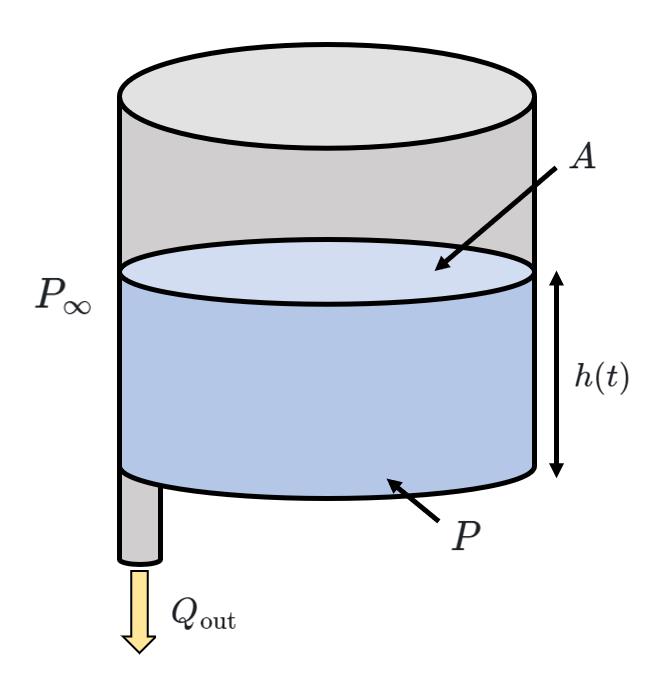
\includegraphics[width=0.65\textwidth,height=\textheight]{figs/2_tank.png}

}

\end{figure}

First off, because the tank is cylindrical, it's apparent that the
volume \(V(t)\) of water in the tank is proportional to the value of
\(h(t)\).

\[V(t) = A h(t)\]

Because of conservation of mass, we know the rate at which the volume is
changing is the difference between the inflow and the outflow.

\[\frac{d}{dt} V(t) = \dot{V} = 0 -Q_\text{out} = -Q_\text{out} \tag{1}\]

That's not very useful yet. Let's leverage some prior circuits knowledge
here\ldots charge moves because of a voltage difference \(\Delta V\),
and comparably, fluid moves because of a pressure difference.\footnote{\(V\)
  refers to voltage here, and not volume as previously defined. This
  contingency also holds true for Ohm's law as defined below.} Ohm's
law! We'll come back to that, but the main takeaway here is that the
volumetric outflow \(Q_\text{out}\) is related to the difference between
the pressure inside the tank \(P(t)\) and the atmospheric pressure
\(P_\infty\) by a ``resistance'' value \(R\).

That circuits analogy comes in handy really often, because it turns out
Ohm's law translates directly into fluid flow.

\[\Delta V = V - V_0 = IR\]
\[\Delta P = P(t) - P_\infty = Q_\text{out} R \tag{2}\]

These are called \textbf{constitutive equations}, or relationships
between physical quantities that establish a connection between a
material's internal response (like stress, strain, or deformation) and
the external factors that influence it (like temperature, pressure, or
applied loads).

We'll generalize a bit soon, but for now I understand if you don't get
it. It's still very hand-wavey.

Let's leverage some hydrostatics now. Assuming the tank is open to the
atmosphere at the top, we can derive an expression for \(\Delta P\)
using the hydrostatic pressure equation \(\Delta P = \rho g \Delta h\).

\[\Delta P = P(t) - P_\infty = \rho g \left(h(t) \right) = \frac{\rho g V}{A}\tag{3}\]

Differentiating equation (3) yields the following.\footnote{Note that
  the derivative of \(\Delta P\) is equal to the derivative of \(P(t)\),
  because \(P_\infty\) is constant.}

\[ \Delta \dot{P}  = \frac{\rho g \dot{V}}{A} \]

Using equations (1) and (2), we can manipulate this equation into a
differential equation in terms of pressure differences.

\[ \Delta \dot{P} = \frac{\rho g \left(- Q_\text{out} \right)}{A} = \frac{- \rho g \Delta P}{A R}\]

\[\Delta \dot{P} + \frac{\rho g}{A R} \Delta P = 0\]

\[R \left( \frac{A}{\rho g}\right) \Delta \dot{P} + \Delta P = 0\]

This is a neat little differential equation. It looks like the equation
for an RC circuit if you've seen those before, with the voltage
differences swapped out for pressure differences. To really drive this
comparison home, we define a ``capacitance'' \(C = \frac{A}{\rho g}\)
and slot it into our governing equation.

\[\boxed{RC \Delta \dot{P} + \Delta P = 0}\]

Perfect. Note that this isn't the only possible governing equation of
the system - it's also possible to find a differential equation in terms
of volume \(V(t)\). Give it a go!

Let's move onto a second example: the cooling of a lightbulb. When we
shut off power to the lightbulb, how can we measure its temperature as
it cools to room temperature?

\begin{figure}

{\centering 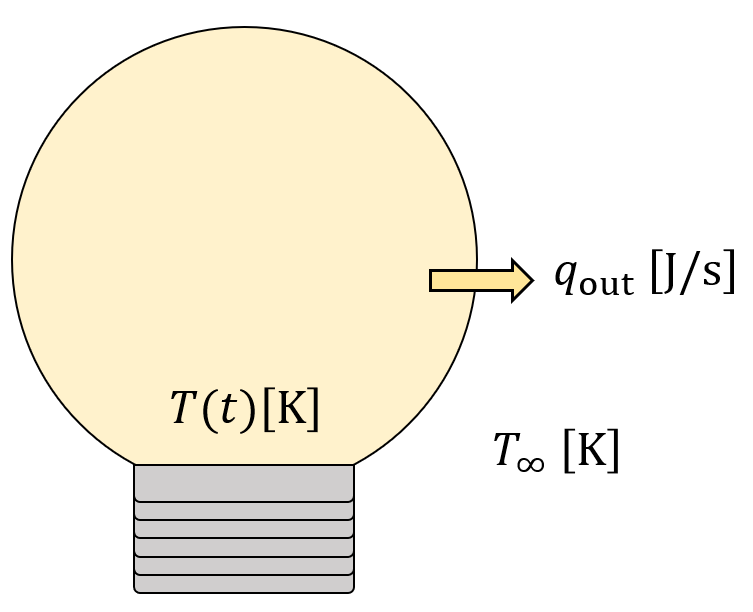
\includegraphics[width=0.65\textwidth,height=\textheight]{figs/2_bulb.png}

}

\end{figure}

The bulb is initially very hot (with temperature \(T\)) compared to its
environment (which has temperature \(T_\infty\)). Heat is flowing
outwards at \(q_\text{out}\). This is seeming very familiar\ldots a
temperature difference is driving heat to leave through the resistance
\(R\) of the bulb.

Let's go through the steps again. Energy's being conserved here, so we
use the capacitive relationship relating accumulated heat \(Q\) and
temperature \(T\) from ESC330:

\[ Q = C \Delta T\]

Differentiate across the board\ldots{}

\[ \dot{Q} = -q_\text{out} = C \Delta \dot{T} \]

And now we're just chugging through the motions. Next is another
constitutive relationship (which looks shudderingly close to Ohm's
law!):

\[\Delta T = T - T_\infty = q_\text{out} R\]

We combine the last two equations and construct:

\[\boxed{RC \Delta \dot{T} + \Delta T = 0}\]

Which surprisingly, just looks like the equation from the first problem.

Ok, one more problem. Say we have an RC circuit - specifically, the
variant where a resistor and a fully charged capacitor are connected in
series without a attached voltage source.

\begin{figure}

{\centering 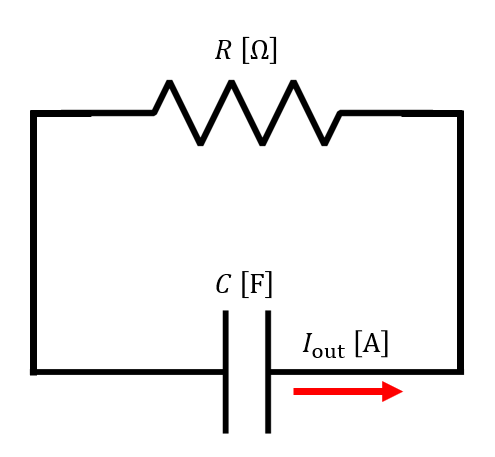
\includegraphics[width=0.65\textwidth,height=\textheight]{figs/2_circ.png}

}

\end{figure}

As we've done twice before, we leverage physical principles to generate
a governing equation for this system. Let's start with conservation of
charge: \[\dot{q} = -I_\text{out}\]

Next, Ohm's law: \[\Delta V = I_\text{out} R = -\dot{q} R\]
\[\dot{q} = -\frac{\Delta V}{R}\]

Finally, we deal in the capacitive relationship: \[q = C\Delta V\]

Manipulating these equations as we did before yields the following
governing equation:

\[C \Delta \dot{V} = -\frac{\Delta V}{R}\]
\[\boxed{RC \Delta \dot{V} + \Delta V = 0}\]

All right, so all of these equations look really similar. What can we
take away from this?

\textbf{Gradients make stuff flow.}

That's a really powerful statement\ldots to those who understand it.
Let's go through it piece by piece.

We define a \textbf{gradient} as a change in the magnitude of a
potential observed at two different points. Some examples of potentials
are:

\begin{itemize}
\tightlist
\item
  Temperature
\item
  Voltage
\item
  Displacement
\item
  Species concentration
\end{itemize}

When a potential difference exists, ``stuff'' has a tendency to move.
For example, when a temperature difference exists across a structure,
heat will flow through it.

``Stuff'' isn't the greatest word for something like this, (maybe
``quantity'' instead?) but to the best of my knowledge, a better word
doesn't exist. We define ``stuff'' as something that can be stored, like
charge in a capacitor, or fluid in a tank, or heat in a reservoir.

By generalizing these quantities, we can create widely applicable rules
for modeling first order systems without having specific knowledge about
the underlying physics.

\[\text{Stuff} = \text{Capacitance} \times \text{Gradient}\]
\[\text{Gradient} = \text{Flow of Stuff} \times \text{Resistance}\]

Also conservation. That's a big one.
\[\text{Rate of Change of Stuff} = \text{Inflow} - \text{Outflow}\]

\hypertarget{the-time-constant}{%
\section{The Time Constant}\label{the-time-constant}}

All of the governing equations we've derived thus far have been of the
form \(\tau \dot{y} + y = 0\). This form, also called the
\textbf{canonical form}, is useful for understanding the behavior of the
dynamic system.

To solve this differential equation, we'll guess a solution
\(y(t) = ce^{\alpha t}\), find its time derivative
\(\dot{y}(t) = \alpha ce^{\alpha t} = \alpha y\), and plug in.

\[\tau \dot{y} + y = 0\] \[\tau \alpha e^{\alpha t} + e^{\alpha t} = 0\]
\[(\tau \alpha + 1) \; e^{\alpha t} = 0\] \[\alpha = -\frac{1}{\tau}\]
\[y(t) = ce^{-\frac{t}{\tau}}\]

Let's toss in an initial condition \(y(0)=y_0\) to get rid of that
unknown constant.

\[y(t) = y_0 \; e^{-\frac{t}{\tau}}\]

We call \(\tau\) the \textbf{time constant} of the system.\footnote{\(\tau = RC\)
  always has units of time.} The time constant of a system is used to
describe how quickly the system response grows or decays. The smaller
the time constant, the faster the decay.

\begin{figure}

{\centering 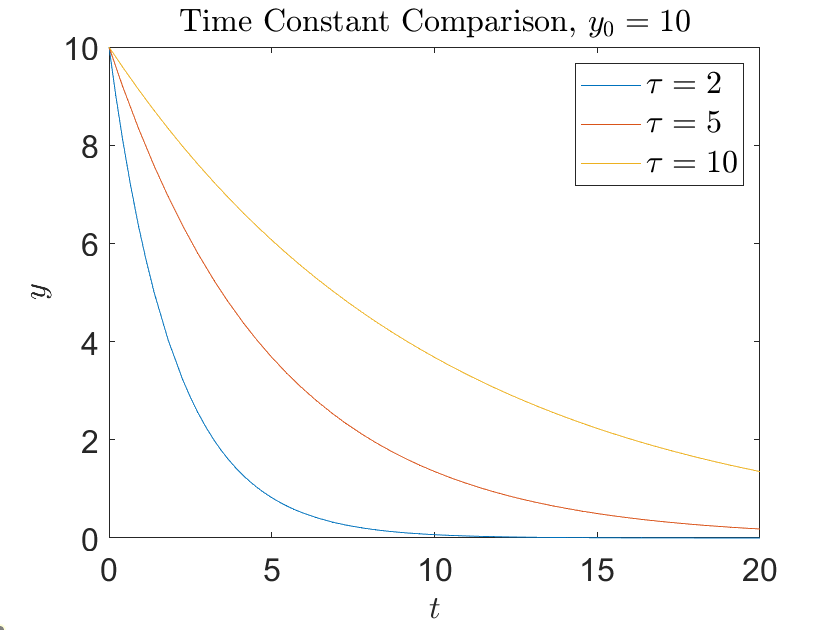
\includegraphics[width=0.75\textwidth,height=\textheight]{figs/2_tc.png}

}

\end{figure}

So what happens when we set \(t=\tau\)?

\[y(\tau) = y_0 e^{-\frac{\tau}{\tau}} = y_0 e^{-1}\]

The time constant is the time at which the system response has decayed
to \(y_0 e^{-1}\), or approximately 37\% of its initial
value.\footnote{Or alternatively, ``the time constant is the time at
  which the system response has lost approximately 63\% of its initial
  value''.}

\hypertarget{lets-throw-in-an-input}{%
\section{Let's Throw in an Input}\label{lets-throw-in-an-input}}

We return to the RC circuit, but this time, let's say there \emph{is} a
voltage source with voltage \(V_\text{s}\). The capacitor initially has
a voltage of \(V_0\), and as time passes, it will charge up through the
resistor until it reaches the supply voltage of the source. (We define
the voltage across the capacitor as \(V_c(t)\).)

\begin{figure}

{\centering 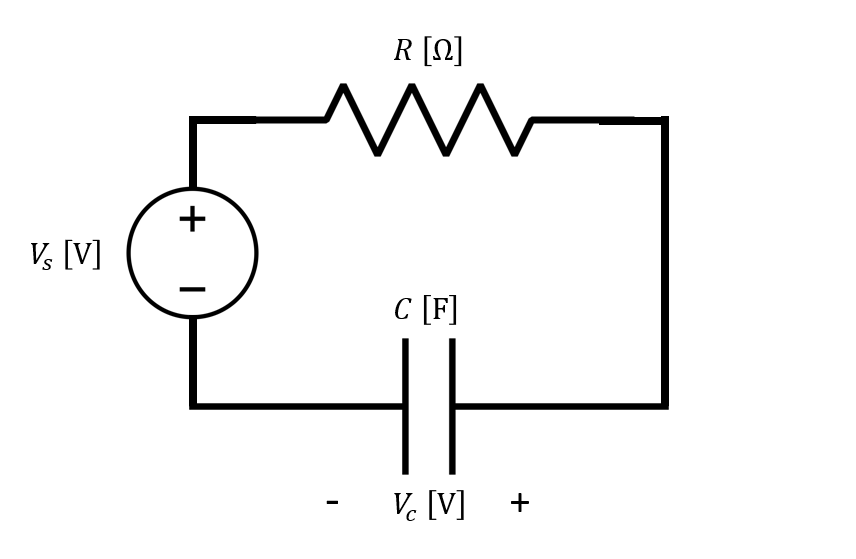
\includegraphics[width=0.65\textwidth,height=\textheight]{figs/2_circ2.png}

}

\end{figure}

To expedite calculations, we'll use Kirchhoff's current law to find a
governing equation for this scenario.

\[ C \dot{V_c} + \frac{V_c - V_s}{R} = 0 \]
\[ RC \dot{V_c} + V_c = V_s \]

That's\ldots different. This equation is no longer homogeneous, meaning
we can't rely on our exponential function guess method anymore. We'll
have to use more specialized methods from Ma240 instead of guessing and
praying, like the method of undetermined coefficients or the Laplace
transform if initial conditions are provided.

A more general form of this governing equation for one of these systems
is:

\[\tau \dot{y} + y = u\]

where \(u\) represents a general input, constant or otherwise. For
example, in the case that the voltage source is an alternator, \(V_s\)
could be a sinusoidal function rather than a constant.

This feels like a good time to introduce the concept of the \textbf{unit
step function}, which I'll denote \(u_s(t)\). The unit step function is
defined as follows:\footnote{We don't care about what happens at
  \(t=0\). Stop it.}

\begin{equation*}
        u_s(t) = \begin{cases}
                        1 &t>0 \\
                        0 &t<0
                    \end{cases}
\end{equation*}

The unit step function is useful for physical modeling because it can be
used to model situations where something changes rapidly from one value
to another. (For example, the unit step function can be used to model
the action of turning on a light switch at time \(t=0\), where 0
represents the light being off and 1 represents the light being on!).

A general form of the governing equation when the input is constant is:

\[\tau \dot{y} + y = ku_s\]

where \(k\) is an arbitrary scale factor. Solving this equation yields:

\[y(t) = ce^{-\frac{t}{\tau}} + k\]

For the initial condition \(y(0) = y_0\), the constant \(c=y_0 - k\).
Here's our updated solution:

\[y(t) = y_0 e^{-\frac{t}{\tau}} + k(1-e^{-\frac{t}{\tau}})\]

When we graph this function for \(y_0 = 0\), we see that it gradually
grows towards \(y=k\) as \(t\to\infty\). Now we can analyze exponential
growth - you see this behavior everywhere, like when you change a
thermostat setting and the temperature slowly creeps towards your
choice. The response of a system in the time domain when the input is
switched from 0 to 1 very quickly is called a \textbf{step response}.

How could we find the time constant of this response? Let's take a look
at what happens to \(y(t)\) at \(t=\tau\).

\[y(\tau) = y_0 e^{-\frac{\tau}{\tau}} + k(1-e^{-\frac{\tau}{\tau}})= y_0 e^{-1} + k(1-e^{-1})\]

When we set \(y_0 = 0\), this further simplifies to:

\[y(\tau) = k(1-e^{-1}) \approx 0.63 k\]

For this system, at \(t=\tau\), the system response will have
accumulated 63\% of its steady state value.

The step input is just one of the test inputs we usually use; we'll look
at a few more as the course progresses (such as sinusoidal waves, delta
functions, etc.).

\bookmarksetup{startatroot}

\hypertarget{our-second-order-of-business}{%
\chapter{Our Second Order of
Business}\label{our-second-order-of-business}}

\hypertarget{preface-1}{%
\section*{Preface}\label{preface-1}}
\addcontentsline{toc}{section}{Preface}

\markright{Preface}

First order systems aren't that interesting. They exhibit a
certain\ldots simplicity in their response to a step input,
characterized by pure exponential behavior. (However, it's important to
appreciate the fundamental nature of this behavior, as it lays the
foundation for understanding more complex dynamic systems.)

Nevertheless, first order systems lack the necessary components to
sustain oscillatory behavior\ldots which really stinks because
oscillation represents a fundamental behavior observed in many natural
and engineered systems.

Second order systems, on the other hand, \emph{can} oscillate by
themselves. \footnote{Try to convince yourself of this mathematically
  just based on what oscillation is.}

Mass-spring systems are pretty versatile models for a really wide range
of phenomena (as long as you use enough mass-spring systems). They're
really nice because having a good understanding of ONE mass-spring
system provides us with the intuition for more complicated systems.
While mass-spring systems may not capture \emph{all} the intricacies and
complexities of real-world phenomena, they serve as an invaluable tool
for providing a framework for understanding a LOT of systems.

\hypertarget{mass-and-spring}{%
\section{Mass and Spring}\label{mass-and-spring}}

\begin{figure}

{\centering 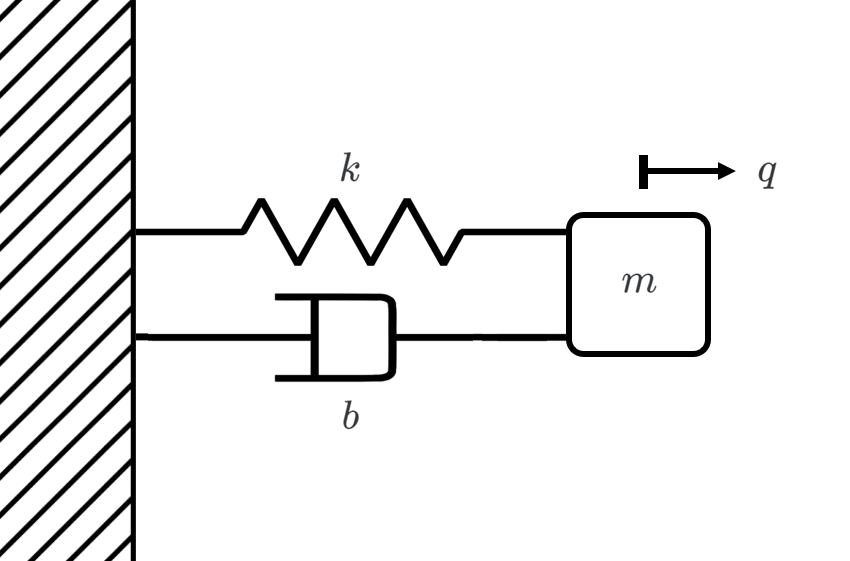
\includegraphics[width=0.65\textwidth,height=\textheight]{figs/3_msd.png}

}

\end{figure}

Say we have a mass-spring system where a mass \(m\) is attached to a
wall with a spring with spring constant \(k\) and a dashpot with damping
coefficient \(b\), as pictured above. (Gravity isn't ``turned on'' in
this scenario.) The equation of motion for a positive displacement \(q\)
is:

\[ ma = \sum F \] \[m\ddot{q} = -kq - b\dot{q}\]
\[m\ddot{q} + b\dot{q} + kq = 0\]

This is a linear differential equation, so we're able to solve this
pretty easily. We'll assume a solution of the form \(q(t) = Ae^{st}\),
where \(A\) is a constant to be determined.
\[m \left( s^2 Ae^{st} \right) + b \left( sAe^{st} \right)+ k \left(Ae^{st} \right)= 0\]

Cancelling out the common term \(Ae^{st}\), we get:

\[ms^2 + bs + k = 0\]

This is known as the \textbf{characteristic (or auxiliary) equation}. We
can solve this quadratic equation to find the values of \(s\), which are
also known as the \textbf{poles} of the system.

\[s_{1, 2} = \frac{-b \pm \sqrt{b^2 - 4mk}}{2m}\]

We can simplify this expression further by defining the \textbf{natural
frequency} \(\omega_n = \sqrt{\frac{k}{m}}\) and the \textbf{damping
ratio} \(\zeta = \frac{b}{2m\omega_n}\). With these definitions, the
poles can be written as:

\[s_{1, 2} = -\zeta \omega_n \pm \omega_n \sqrt{\zeta^2 - 1}\]

In terms of the variables \(\zeta\) and \(\omega_n\), the mass-spring
equation can be rewritten as:

\[\ddot{q} + 2\zeta\omega_n \dot{q} + \omega_n^2 q = 0\]

The damping ratio \(\zeta\) and the natural frequency \(\omega_n\)
provide important insights into the behavior of the system. However,
note that the value of \(\zeta\) is crucial in determining the nature of
the poles of the system; it directly affects whether they're real or
imaginary.

Before we deal with that, though, I'll introduce some technology from
complex analysis to make our lives a bit easier.

\begin{center}\rule{0.5\linewidth}{0.5pt}\end{center}

Complex analysis is the study of functions of a complex variable \(z\),
where \(z\) has a real component \(a\) and an imaginary component \(b\).
Complex numbers show up all the time in this course, whenever anything
oscillates, really (like mass-spring systems or pendulums).

To take our first plunge into complex analysis, we need to define the
\textbf{imaginary unit} \(i\).\footnote{Prof.~Baglione likes to comment
  that mathematicians use \(i\) and engineers use \(j\), which is pretty
  funny. Usually, \(j\) is used by electrical engineers for
  disambiguation with current, which is often represented with an \(i\)
  as well.} \(i\) is a number that satisfies the equation \(i^2 = -1\).
Since the square of any real number is always non-negative, there is no
real number that safisties this equation. Thus, \(i\) is considered an
imaginary number. (Ooh!)

Recall from algebra that every non-constant polynomial over
\(\mathbb{R}\) can be factored into linear and quadratic terms. Any real
quadratic can be factored into linear terms over \(\mathbb{C}\), the set
of all complex numbers. As such, \(\mathbb{C}\) has the roots of all
polynomials over \(\mathbb{R}%
\).

This is really special - in other words, every polynomial of degree
\(n\) has \(n\) complex roots, counting multiplicity. This is known as
the Fundamental Theorem of Algebra - it's a nice thing to stash in the
back of your head, and it'll come back in a bit.

Let's conjure up a graphical representation of these complex numbers
using Cartesian coordinates, where the real numbers are represented
along the \(x\)-axis and the imaginary numbers along the \(y\)-axis.
We'll call this the complex plane.

In this representation, a complex number \(z = a + bi\) can be
visualized as a point in the two-dimensional Cartesian plane, with the
real part \(a\) as the \(x\)-coordinate and the imaginary part \(b\) as
the \(y\)-coordinate.

\begin{figure}

{\centering 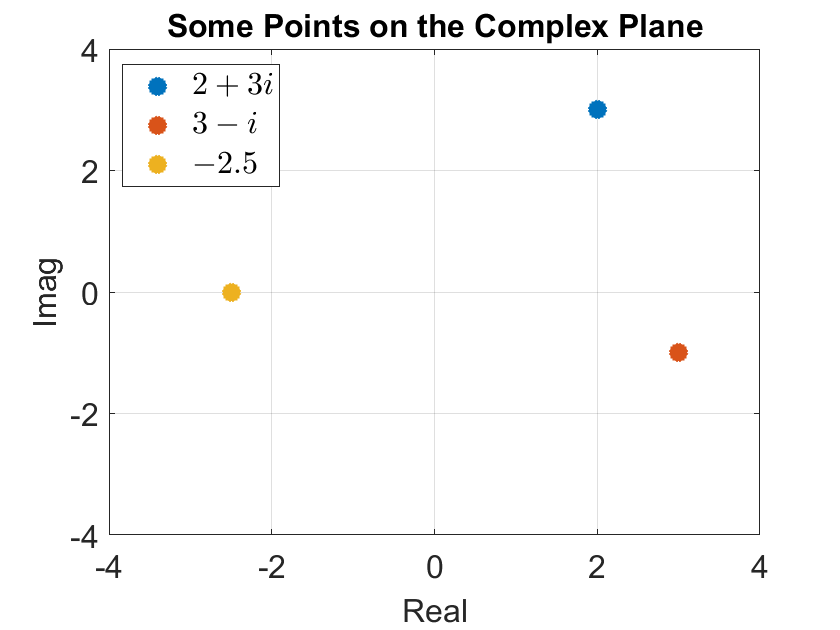
\includegraphics[width=0.65\textwidth,height=\textheight]{figs/3_poles.png}

}

\end{figure}

By plotting these complex numbers on the plane, we can observe their
geometric relationships. Additionally, algebraic operations can be
understood in terms of vector addition, subtraction, and scalar
multiplication.

Complex numbers can also be interpreted in the context of polar
coordinates - in polar coordinates, a complex number \(z = a + bi\) is
described by two quantities: the magnitude \(r\) and the argument
\(\theta\). The magnitude \(r\) represents the distance from the origin
\((0,0)\) to the point representing the complex number \(z\) in the
complex plane. It's calculated using the Pythagorean theorem:

\[r = \sqrt{a^2+b^2}\]

The argument, denoted as \(\theta\), represents the angle between the
vector from the origin to \(z\) and the positive real axis, measured
counterclockwise. The argument can be determined as follows (with
additional precautions depending on the quadrant):

\[\theta = \arctan \left( \frac{b}{a} \right)\]

Converting back to Cartesian coordinates is trivial.

\[a = r \cos{\theta} \qquad \qquad b = r \sin{\theta}\]

It'd be criminal to not mention Euler's formula, which connects
trigonometric functions to the complex exponential: \footnote{You can
  prove this by substituting \(x = i \theta\) into the Taylor series
  expansion of \(e^{x}\). Do it, it's \emph{very} rewarding.}

\[e^{i\theta} = \cos{\theta} + i \sin{\theta}\]

This result demonstrates the connection between exponentials and
trigonometric functions, bringing together complex numbers, angles, and
the unit circle. It also means that we can express complex numbers in
the elegant form:

\[z = a+bi = r\cos{\theta} + i r \sin{\theta} = r (\cos{\theta} + i \sin{\theta}) = re^{i\theta}\]

This is \emph{really} useful. It simplifies complex number arithmetic,
enables efficient calculations of powers and roots, and provides a
natural framework for solving differential equations involving complex
variables.

\begin{center}\rule{0.5\linewidth}{0.5pt}\end{center}

Phew. Okay, back to springs.

We know from our study of differential equations that \(q = e^{st}\) is
a solution of the equation when \(s\) is a pole of the system. Let's
break each possibility down case by case.

When \(\zeta = 0\) (or when the system is \textbf{undamped}), the poles
are:

\[s_{1, 2} = -\zeta \omega_n \pm \sqrt{\omega_n^2 (\zeta^2 - 1)} = \pm \sqrt{-\omega_n^2 } = \pm i \omega_n\]

And the solution is:
\[q(t) = A_1 e^{i\omega_n t} + A_2 e^{- i \omega_n t} = A_1 (\cos(\omega_n t) + i \sin(\omega_n t)) + A_2 (\cos(\omega_n t) - i \sin(\omega_n t))\]
\vspace{-0.3in}
\[= (A_1 + A_2) \cos(\omega_n t) + i(A_1 - A_2) \sin(\omega_n t) = C_1 \cos(\omega_n t) + C_2 \sin(\omega_n t)\]

Physically, when a mass-spring damper system is undamped, the mass will
oscillate forever.

When we pick a damping ratio \(\zeta\) between 0 and 1 (or the system is
\textbf{underdamped}), the poles are:

\[s_{1, 2} = -\zeta \omega_n \pm \sqrt{\omega_n^2 (\zeta^2 - 1)} = -\zeta \omega_n \pm i \omega_n \sqrt{1 - \zeta^2}\]

We further consolidate the definition of these poles using two
additional definitions: we define the \textbf{damped frequency}
\(\omega_d = \omega_n \sqrt{1-\zeta^2}\), and a ``growth parameter''
\(\sigma = \zeta \omega_n\).\footnote{Not sure if there's an agreed upon
  name for this value, but I think that term covers the necessary bases.}
These result in a more concise representation of the poles:

\[s_{1, 2}  = - \sigma \pm i \omega_d \]

Our solution, given these poles, is:
\[q(t) = A_1 e^{(-\sigma + i\omega_d) t} + A_2 e^{(-\sigma - i\omega_d) t} = e^{-\sigma t} (C_1 \cos(\omega_n t) + C_2 \sin(\omega_n t))\]

Representing the solution as a product of a real exponential and a
linear combination of sines and cosines allows us to characterize the
exponential \textbf{envelope} by which the oscillation decays. An
envelope is a function that outlines the extremes of a function. The
figure below shows a sinusoidal wave and its upper envelope.

\begin{figure}

{\centering 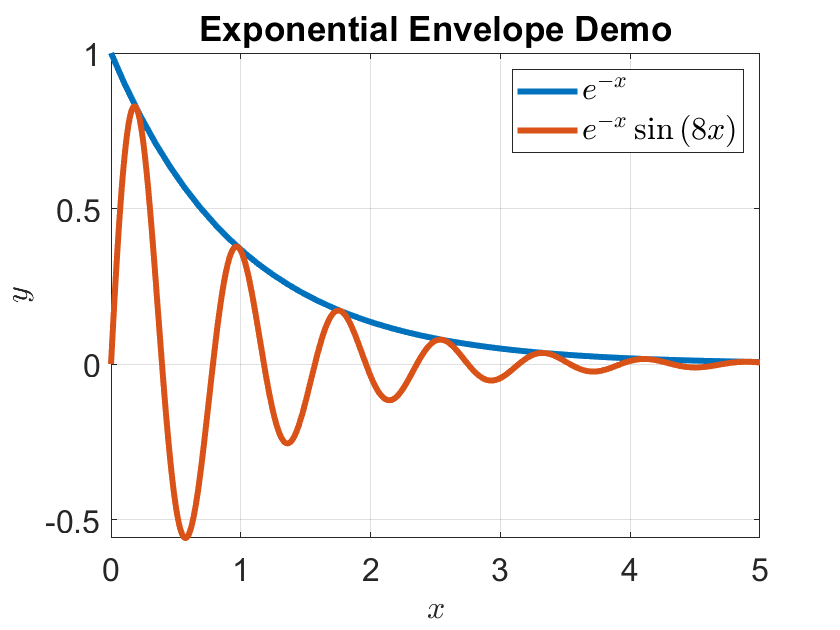
\includegraphics[width=0.65\textwidth,height=\textheight]{figs/3_env.png}

}

\end{figure}

Notably, the time constant \(\tau\) of the envelope is equal to
\(1/\sigma\). Thus, we can eyeball the value of \(\sigma\) based on how
we'd find the time constant (the value \(63\%\) less than the
\(y\)-intercept of the envelope).
\[q(t) = e^{-\sigma t} \sin(\omega_d t + \varphi)\]

Most mechanical systems tend to have a pretty low damping ratio
(\(\zeta \simeq O(0.1)\)),\footnote{This notation just means ``on the
  order of''.} and a good rule of thumb is that \(\omega_n = \omega_d\).

When \(\zeta = 1\), or the system is \textbf{critically damped}, the
poles are:

\[s_{1, 2} = -\zeta \omega_n = - \sigma\]

We use a trick from differential equations to fake another linearly
independent solution, just chuck on an extra \(t\).

\[q(t) = A_1 e^{-\zeta \omega_n t} + A_2 t e^{-\zeta \omega_n t} = A_1 e^{-\sigma t} + A_2 t e^{-\sigma t}\]

This doesn't really happen in the real world, but it's nice to cover all
our bases - how about the case where \(\zeta > 1\)? The system is
\textbf{overdamped} and our poles are:

\[s_{1, 2} = -\zeta \omega_n \pm \omega_n \sqrt{\zeta^2 - 1}\]

Both poles are negative here! Our solution is:

\[q(t) = A_1 e^{s_1 t} + A_2 e^{s_2 t}\]

Overdampedness implies that the mass can slowly return to equilibrium
without ever overshooting as it would in the underdamped case.

\begin{figure}

{\centering 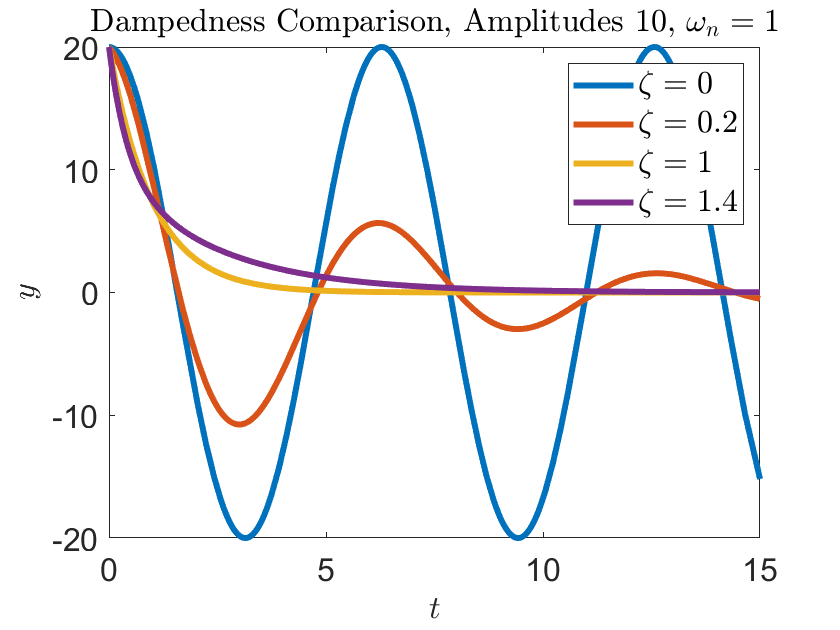
\includegraphics[width=0.65\textwidth,height=\textheight]{figs/3_damp.png}

}

\end{figure}

\hypertarget{leveraging-the-discriminant}{%
\section{Leveraging the
Discriminant}\label{leveraging-the-discriminant}}

I'm going to stray off from Prof.~Luchtenburg for a second because
\emph{I} think this is really useful.

Suppose we want to identify the dampedness of a system immediately based
on the equation of motion rather than solving for \(\zeta\). We can do
exactly this using the \textbf{discriminant} of the characteristic
equation of the system. Let's take a look at the canonical mass-spring
system with a damper once again.

The equation of motion, assuming free motion, is:
\[m\ddot{q} + b \dot{q} + k q = 0\]

The characteristic equation is derived after plugging in \(q = e^{st}\).
\[ms^2 + bs + k = 0\]

As stated in the section on damping, there are three forms of the
general solution if there is damping present: both poles are real and
distinct (the system is overdamped), both poles are real and equal (the
system is critically damped), or both poles are complex conjugates (the
system is underdamped). You may recall from algebra that the
discriminant of a polynomial can reveal some properties of the roots
without having to compute them. The discriminant of a quadratic is
defined as follows: \[\text{Disc}(ax^2 + bx + c) = b^2-4ac\]

Notably, this is the argument of the square root in the quadratic
formula. If this expression is positive, the solutions to the quadratic
are real and distinct. If this expression is 0, then there is only one
real solution to the quadratic. If this expression is negative, the
solutions to the quadratic are complex. So physically, finding the
discriminant of the characteristic equation of the mass-spring system
will tell us how damped it is. \[\text{Disc}(ms^2 + bs + k) = b^2-4mk\]

\begin{align*}
    b^2 - 4mk > 0 \quad &\to \quad \text{overdamped} \\
    b^2 - 4mk = 0 \quad &\to \quad \text{critically damped} \\
    b^2 - 4mk < 0 \quad &\to \quad \text{underdamped}
\end{align*}

And of course, if \(b=0\), then the system is undamped.

\hypertarget{pole-plots}{%
\section{Pole Plots}\label{pole-plots}}

We use a graphical tool called a \textbf{pole plot}, the plot of the
roots of the characteristic equation on the complex plane, to determine
the dampedness of a system from its poles. Let's go down the list:

\begin{itemize}
\tightlist
\item
  When both poles are on the imaginary axis, the system is undamped.
\item
  When both poles are off the real axis, the system oscillates. If
  they're to the left of the imaginary axis, it'll decay exponentially
  (underdamped), and if they're to the right of the imaginary axis,
  it'll grow exponentially.
\item
  If both poles are on the real axis to the left of the imaginary axis,
  it's overdamped.
\item
  Rule of thumb: if there is ANY pole to the right of the imaginary
  axis, the response blows up.
\end{itemize}

Here's a nice chart from FPE. Complex conjugates are omitted for
simplicity.

\begin{figure}

{\centering 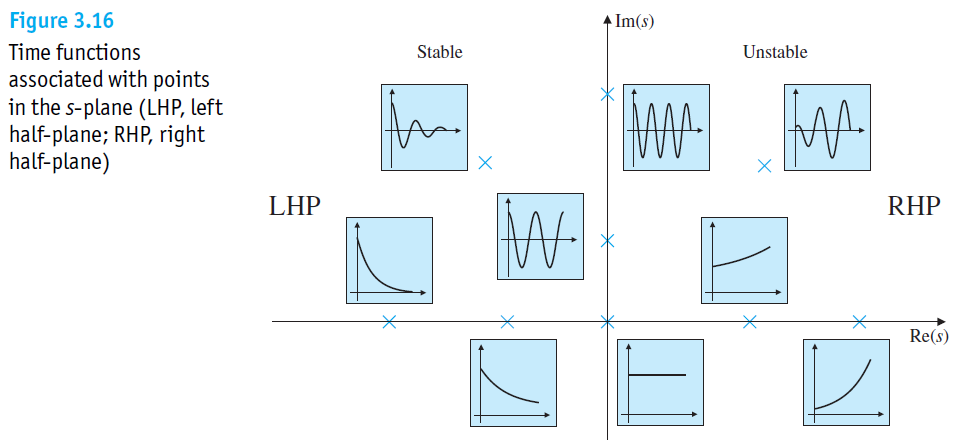
\includegraphics[width=0.75\textwidth,height=\textheight]{figs/3_pol.png}

}

\end{figure}

\hypertarget{the-dominant-pole-approximation}{%
\section{The Dominant Pole
Approximation}\label{the-dominant-pole-approximation}}

The concept of pole ``speed'' is often useful when analyzing higher
order systems. While we're able to gather valuable information from
first and second order systems, doing this for systems of a higher order
is more complicated.

A technique called the \textbf{dominant pole approximation} is
applicable in these cases - namely, in the case that poles are
substantially far apart, the slowest part of a system ``dominates'' the
response and the faster parts are negligible for analysis.

It's better to explain by showing rather than telling here. Say we're
provided with the following third order system (I don't know, like
hurricane wind):

\[ \frac{d^3 x}{dt^3} + 110.1 \frac{d^2 x}{dt^2} + 1011 \frac{d x}{dt} + 100x = u \]

The characteristic equation, expressed in terms of \(s\), is:

\[ s^3 + 110.1 s^2 + 1011 s + 100 = (s+0.1)(s+10)(s+100) = 0 \]

This equation has the roots \(-0.1\), \(-10\), and \(-100\). By
definition, these are the poles of our system.

Poles closer to the origin (in this case, \(s=-0.1\)) are considered
\textbf{slower} than those farther away from the origin. This
approximation poses that the slowest part of the system dominates the
response, and that the effect of the faster poles can be ignored. (This
is of course only the case if the gap between the slowest part of the
system and the faster part(s) is large enough - this is, of course, just
an approximation.)

Let's continue with this problem. The slowest pole here is \(s=-0.1\),
so we assume that the response to:

\[ \frac{d^3 x}{dt^3} + 110.1 \frac{d^2 x}{dt^2} + 1011 \frac{d x}{dt} + 100x = u \]

is similar to that of:

\[ 1000 \left( \frac{d x}{dt} + 0.1 x \right) = u \]

The scale factor of 1000 is necessary for the approximation - since we
want the final value of the response to remain unchanged, we apply the
additional condition that when all derivatives are zero, the original
system and the approximation should be the same.\footnote{I'm really
  dancing around poles, transfer functions, and the Final Value Theorem
  here so I might write a follow-up section to this in Chapter 6 when
  we've developed the technology for it.}

\begin{figure}

{\centering 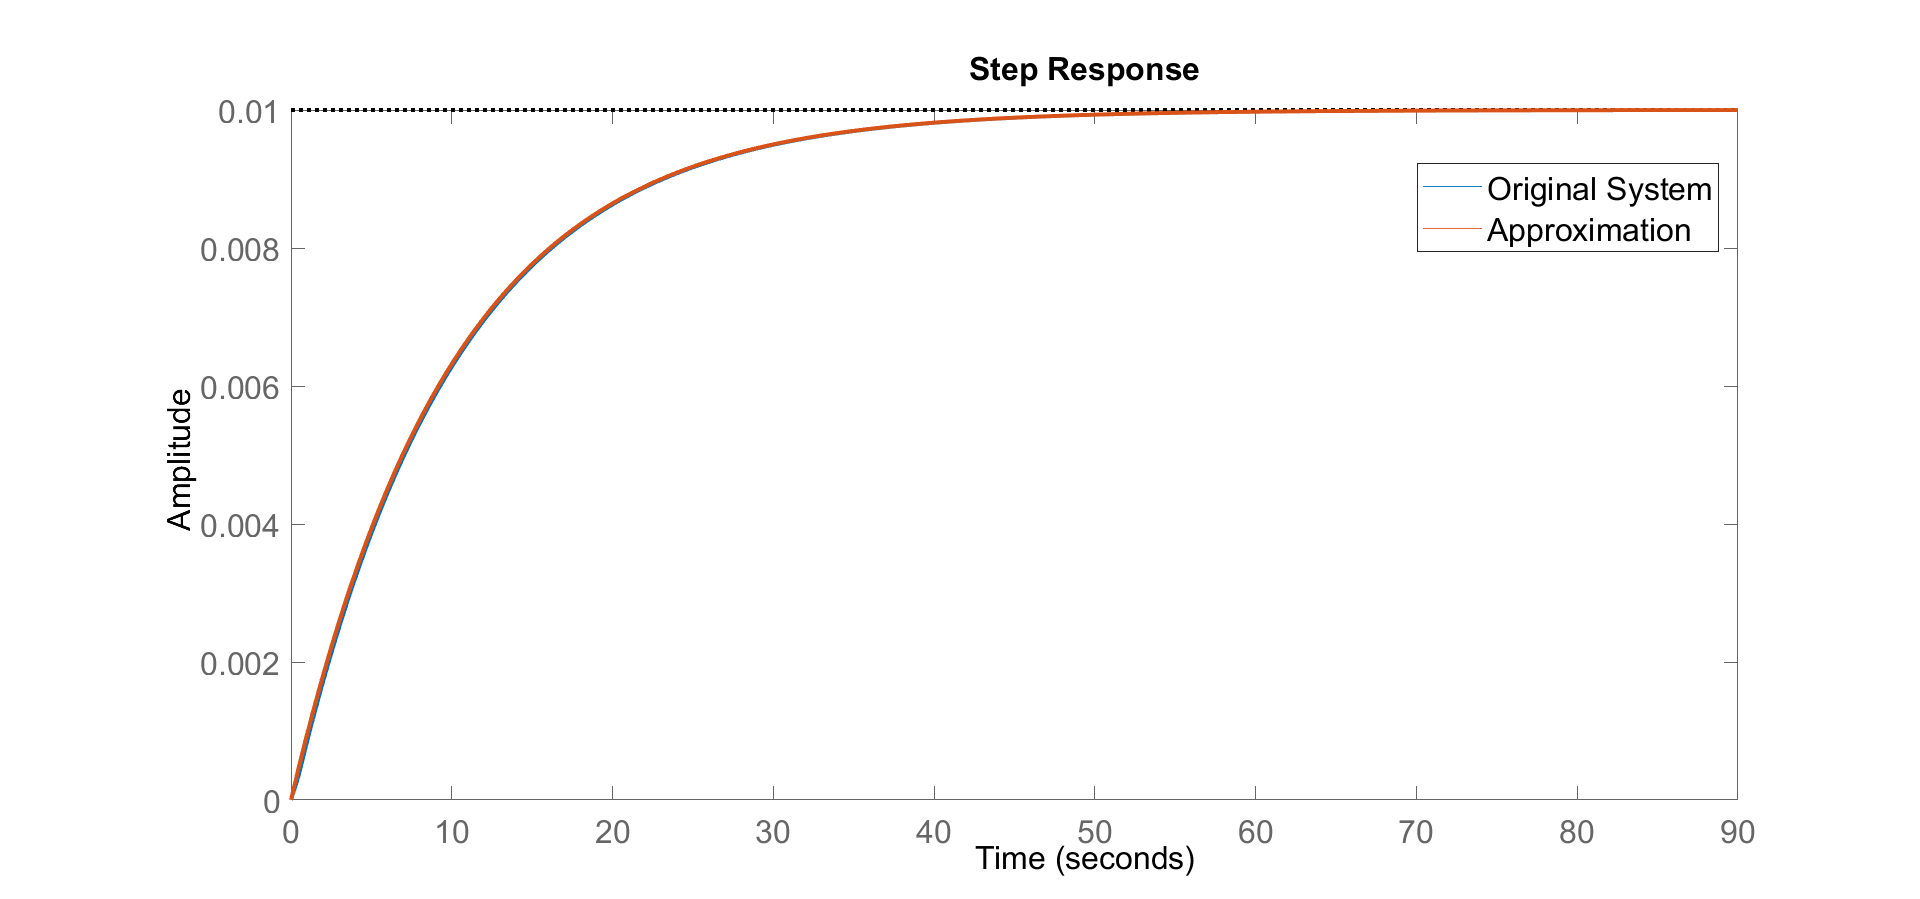
\includegraphics[width=0.85\textwidth,height=\textheight]{figs/3_approx.png}

}

\end{figure}

This approximation can also work for systems with complex poles - we can
quantify a pole's speed based on their real component.

Remember that this is just an approximation. There are times when it's
very cool and sleek to boot out a bunch of poles, but sometimes you're
losing valuable information about a system's dynamic behavior.
Prof.~Fontaine says something that fits this situation pretty well in
his Signal Processing class -

\begin{quote}
Do no harm to the signal. Anything you do harms the signal. Sometimes
the best option is to do nothing.
\end{quote}

\hypertarget{the-tank-revisited-inertia}{%
\section{The Tank, Revisited
(Inertia)}\label{the-tank-revisited-inertia}}

Let's revisit the tank from our study of first order systems. However,
we'll make one small change: the outflow pipe now has a defined length
of \(L_p\).

\begin{figure}

{\centering 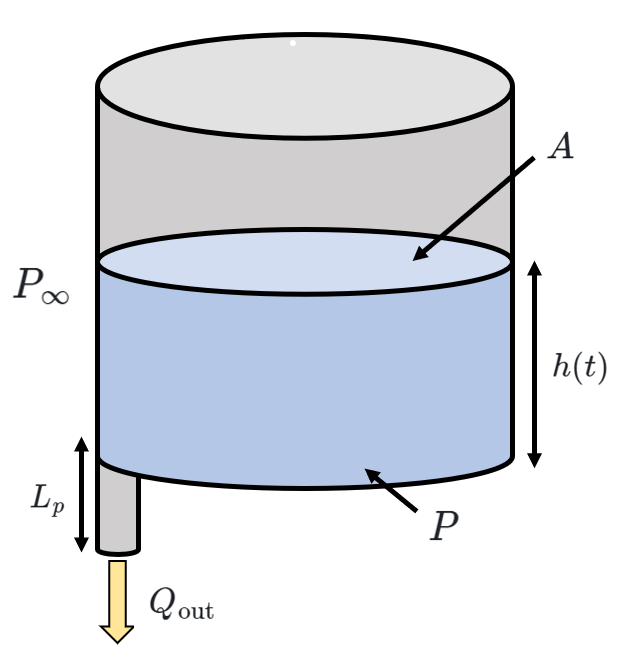
\includegraphics[width=0.65\textwidth,height=\textheight]{figs/3_tank3.png}

}

\end{figure}

We'll model the same way we've been doing thus far. First, a
conservation law:

\[\dot{V} = -Q\]

Next, ``Ohm's law'':

\[Q = \frac{\Delta P}{R} = \frac{P - P_\text{atm}}{R}\]

Let's take a closer look at that pipe.

\begin{figure}

{\centering 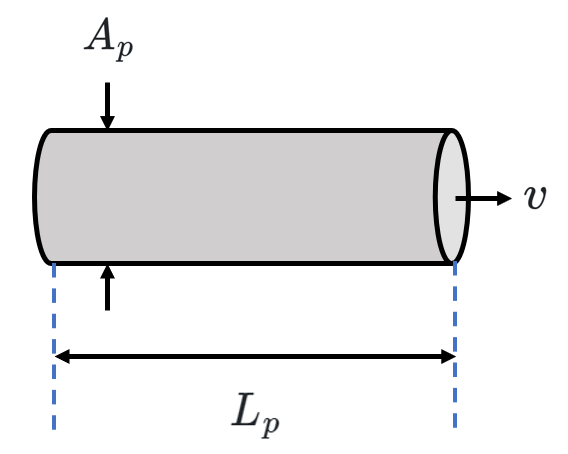
\includegraphics[width=0.55\textwidth,height=\textheight]{figs/3_pipe.png}

}

\end{figure}

Assuming the cross-sectional area of the pipe \(A_p\) is constant, the
pressure force \(F_p = A_p \Delta P\) accelerates the fluid between the
two ends of this pipe. Additionally, there is friction \(F_f = -QRA_p\)
on the liquid caused by the resistance of the pipe. By leveraging
Newton's second law of motion, we now have a relationship between the
pressure difference \(\Delta P\) and the velocity of the water \(v\).

\[m \frac{dv}{dt} = F_p + F_f = A_p \Delta P - Q R A_p\]

The mass \(m\) of the fluid between the two ends of this pipe is equal
to the product of the density of the fluid \(\rho\) and the volume
between the two ends \(V_p\). (Notably, the volume \(V_p = A_p L_p\).)

\[\rho \, V_p \, \frac{dv}{dt} = \rho A_p L_p \, \frac{dv}{dt} = A_p \Delta P - RQ A_p\]

Because the product of the cross-sectional area \(A_p\) and the fluid
velocity \(v\) is equal to the volumetric flow rate \(Q\), we can
rewrite this equation as follows:

\[\frac{\rho L_p}{A_p} \, \frac{dQ}{dt} = \Delta P - RQ\]

Ok, we can shed some light on what we're doing now. We define
\textbf{inductance} (also referred to as \textbf{liquid-flow inertance}
or \textbf{inertia}) as a term that describes the change in potential
required for a unit rate of fluid flow. Inductance is the tendency of
the fluid to move; it's created by the inertia of water flowing through
the pipe. The mathematical definition of inductance is as follows:

\[L = \frac{\rho L_p}{A_p}\]

Note that this definition of inductance is only valid for flow systems,
but analogous concepts occur in other fields (like inductors from
circuit analysis)! Fluid components that have an inductance are
analogous to these inductors, or mechanical components with inertia.

Let's wrap up this example. When we plug in the definition of \(L\) into
our equation, a simple first order system rears its ugly
head.\footnote{The analog of this system in circuit analysis is called
  the RL circuit, which is often used as a passive filter.}

\[L \, \frac{dQ}{dt} + RQ = \Delta P\]

Let's throw it into canonical form so we can see its time constant.

\[\left(\frac{L}{R}\right) \dot{Q} + Q = \frac{\Delta P}{R} \qquad \qquad \tau = \frac{L}{R}\]

To summarize, we've added a new tool to our arsenal: conservation of
momentum (or Newton's second law).

\[\Delta P = L \dot{Q} + RQ\] \[\dot{V} = -Q\] \[C \Delta P = V\]

By combining these three equations, we can use tools from our studies of
mass-spring systems to analyze\ldots{} well\ldots{} any second order
system.

\[L \Delta \ddot{P} + R \Delta \dot{P} + \frac{1}{C} \Delta P = 0 \qquad \to \qquad \Delta \ddot{P} + \left(\frac{R}{L}\right) \Delta \dot{P} + \left(\frac{1}{LC}\right) \Delta P = 0\]
\[m \ddot{q} + b \dot{q} + k q = 0 \qquad \to \qquad \ddot{q} + \left(\frac{b}{m}\right) \dot{q} + \left(\frac{k}{m}\right) q = 0\]

We simply retrofit the definitions of the natural frequency \(\omega_n\)
and damping ratio \(\zeta\) based on how we defined them for mass-spring
systems to determine how the oscillations behave. Here's a quick example
using the flow system scenario we've been tackling thus far:
\[\ddot{q} + 2\zeta\omega_n \dot{q} + \omega_n^2 q = 0 \quad \longleftrightarrow \quad  \Delta \ddot{P} + \left(\frac{R}{L}\right) \Delta \dot{P} + \left(\frac{1}{LC}\right) \Delta P = 0\]

\begin{align*}
    2 \zeta \omega_n = \frac{R}{L} \qquad &\longrightarrow \qquad \zeta = \frac{R}{2L \omega_n} = \frac{R\sqrt{LC}}{2L} = \frac{R}{2} \sqrt{\frac{C}{L}}\\
    \omega_n^2 = \frac{1}{LC} \qquad &\longrightarrow \qquad \omega_n = \frac{1}{\sqrt{LC}} = \frac{\sqrt{LC}}{LC}
\end{align*}

\bookmarksetup{startatroot}

\hypertarget{an-engineering-students-butchering-of-ma326}{%
\chapter{An Engineering Student's Butchering of
Ma326}\label{an-engineering-students-butchering-of-ma326}}

\hypertarget{preface-2}{%
\section*{Preface}\label{preface-2}}
\addcontentsline{toc}{section}{Preface}

\markright{Preface}

This chapter's going to be a smorgasbord of mathematical concepts I
think are foundational to understanding this course from a theoretical
perspective. A decent chunk of it will be review from Ma110 and Ma240,
but it doesn't hurt to take a second look at these things (they keep
coming back over and over). That being said, this chapter largely strays
off from Prof.~Luchtenburg's curriculum, especially in the latter half
of section 4.3.

What I'll try to do, instead of rehashing what you got out of Ma240, is
reframe these concepts in a way that's more applicable to this course
(and ME351). I'll also formalize a bunch of concepts from Ma326 that are
really important to know for this class (and later on). But first, let's
formalize a few more definitions that will come in handy later on.

A \textbf{linear combination} of elements of a set
\(x_1, x_2, ..., x_n\), is given by:

\[a_1 x_1 + a_2 x_2 + ... + a_n x_n \]

where each \(a_i\) is a constant. In layman's terms, a linear
combination of variables is the sum of scaled versions of those
variables, where the scaling factor is a scalar.

A set of variables are \textbf{linearly dependent} if one of the
variables can be expressed as a linear combination of the others. More
formally, a set of variables \(x_1, x_2, ..., x_n\) is linearly
dependent if there exist scalars \(a_1, a_2, ... a_n\) (not all zero),
such that:

\[a_1 x_1 + a_2 x_2 + ... + a_n x_n = 0\]

On the other hand, if no such scalars exist, the set of variables is
said to be \textbf{linearly independent}.

\hypertarget{linearity-and-time-invariance}{%
\section{Linearity and
Time-Invariance}\label{linearity-and-time-invariance}}

A \textbf{linear time-invariant (LTI) system} is a mathematical model
often used in control theory to describe the behavior of physical
systems. It is characterized by two properties: linearity and
time-invariance. I'll describe these separately in the context of
differential equations. A differential equation of the form:

\[a_n y^{(n)} (t) + a_{n-1} y^{(n-1)} + ... + a_1 \dot{y}(t) + a_0 y(t) = f(t)\]

where \(y^{(i)}\) is the \(i\)th derivative of \(y(t)\), is called
\textbf{linear}. (The relationship between \(y(t)\) and \(t\) is a
linear mapping.) A system is linear if and only if it satisfies two
properties: superposition and homogeneity:

\begin{itemize}
\tightlist
\item
  \textbf{Superposition} - if \(x_1 \to y_1\) and \(x_2 \to y_2\), then
  \(x_1 + x_2 \to y_1 + y_2\)
\item
  \textbf{Homogeneity} - if \(k\) is a scalar and \(x \to y\), then
  \(kx \to ky\)
\end{itemize}

If \(\{a_i\}_0^n\), also called coefficients, are constants, the
equation is also characterized as a \textbf{constant coefficient}
differential equation. Physically, constant coefficients imply that the
system behavior does not depend on time.

We can establish an equivalence between linear constant coefficient
equations and linear time-invariant systems. Time-invariance is the
principle that if we chug an input \(t_0\) into a system that outputs
\(y(t_0)\), the input \(t_0 + t_1\) will result in an output of
\(y(t_0 + t_1)\).\footnote{An equivalent definition in signal processing
  is that a system is time-invariant if it commutes with a ``delay''.}

Let's take a look at a few examples to make this more clear:

\[\dot{y} + \sin(t) y = 0\]

This system is not LTI, because the coefficient of \(y\) is not
constant. (More explicitly, it's a function of \(t\), so as
\(t \to \infty\), the behavior is affected.)

\[2 \dot{y} + 3 y = 0\]

This system \emph{is} LTI, because the coefficients of each derivative
of \(y\) are constant.

\[\dot{y} + \ln(y) = 0\]

This system isn't even linear, for obvious reasons.

Examples of LTI systems include first-order passive filters, second
order systems such as springs and masses, and many other linear systems
in control theory and signal processing.

\hypertarget{matrices-at-lightspeed}{%
\section{Matrices, at Lightspeed}\label{matrices-at-lightspeed}}

I truly hope you know what a matrix is by now. If not, fasten your
seatbelt.

A matrix is a rectangular array of numbers, of the form:

\[\textbf{A} = \begin{bmatrix}
    a_{11} & a_{12} & ... & a_{1n}\\ a_{21} & a_{22} & ... & a_{2n}\\ \vdots & \vdots & \ddots & \vdots \\ a_{m1} & a_{m2} & ... & a_{mn}
\end{bmatrix}\]

where \(a_{ij}\) is the entry at row \(i\) and column \(j\). We say a
matrix is of size \(m \times n\), where \(m\) is the number of rows and
\(n\) is the number of columns.

\[\underbrace{\begin{bmatrix}
    1 & 2 \\ 3 & 4 \\ 5 & 6
\end{bmatrix}
}_{3\times 2}\]

Matrices are pretty neat. We can add numbers in the matrix elementwise
and scale it by a scalar factor as follows:

\[\begin{bmatrix}
    a_1 & b_1 \\ c_1 & d_1
\end{bmatrix} + \begin{bmatrix}
    a_2 & b_2 \\ c_2 & d_2
\end{bmatrix} = \begin{bmatrix}
    a_1 + a_2 & b_1 + b_2 \\ c_1 + c_2 & d_1 + d_2
\end{bmatrix}\]

\[ k \begin{bmatrix}
    a & b \\ c & d
\end{bmatrix} = \begin{bmatrix}
    ka & kb \\ kc & kd
\end{bmatrix}\]

The \textbf{zero matrix} \textbf{0} is an \(m\times n\) matrix with all
entries 0. The zero matrix plays an important role in linear algebra, as
it is the additive identity for matrices. This means that adding a zero
matrix to any matrix does not change the matrix, much like adding zero
to any number does not change its value.

A \textbf{square matrix} is a matrix with the same number of rows and
columns. Many concepts in linear algebra are designed with these in
mind, such as determinants and eigenvalues.

Next, we'll tackle the \textbf{Kronecker delta}, which is is a useful
and important symbol in mathematics, particularly in linear algebra and
related fields. Its simple definition allows for the easy expression of
many concepts and operations, making it a valuable tool for
mathematicians and scientists. We define the Kronecker delta
\(\delta_{ij}\) as follows:

\begin{equation*}
    \delta_{ij} = \left\{ \begin{array}{ll}
        1 \quad i=j\\
        0 \quad i \neq j
    \end{array} \right.
\end{equation*}

Following from this, the \textbf{identity matrix} \(\textbf{I}_n\) is
defined as an \(n\times n\) square matrix where
\((\textbf{I}_n)_{ij} = \delta_{ij}\), i.e.,

\[\textbf{I}_1 = 1, \; \textbf{I}_2 = \begin{bmatrix}
    1 & 0 \\ 0 & 1
\end{bmatrix}, \; \textbf{I}_3 = \begin{bmatrix}
    1 & 0 & 0 \\ 0 & 1 & 0 \\ 0 & 0 & 1
\end{bmatrix}, \; ...\]

The set of all matrices fixed at size \(m \times n\) with scalar entries
forms something we call a vector space. There's a lot of nuance attached
to that name; if you care about it, take Ma326. Here are a few
properties for now. (Bolded quantities are matrices, \(a, b,\) and 1 are
scalars.)

\begin{itemize}
\tightlist
\item
  Matrix addition is commutative, i.e.,
  \(\textbf{X} + \textbf{Y} = \textbf{Y} + \textbf{X}\)
\item
  Matrix addition is associative, i.e.,
  \((\textbf{X} + \textbf{Y}) + \textbf{Z} = \textbf{X} + (\textbf{Y} + \textbf{Z})\)
\item
  Each matrix has an additive identity, i.e.,
  \(\textbf{X} + \textbf{0} = \textbf{X}\)
\item
  Each matrix has an additive inverse, i.e.,
  \(\textbf{X} + \textbf{Y} = \textbf{0}\)
\item
  Each matrix has a scalar multiplicative identity, i.e.,
  \(1 (\textbf{X}) = \textbf{X}\)
\item
  \((ab)\textbf{X} = a(b\textbf{X})\)
\item
  \(a(\textbf{X} + \textbf{Y}) = a\textbf{X} + a\textbf{Y}\)
\item
  \((a+b)\textbf{X} = a\textbf{X} + b\textbf{X}\)
\end{itemize}

We can multiply two matrices of sizes \(m\times n\) and \(n\times p\),
respectively, to produce another matrix of size \(m\times p\). The
operation, dubbed \textbf{matrix multiplication}, should not be confused
with the scalar multiplication used before. It's defined as follows:

\[(\textbf{AB})_{ij} = \sum_{k=1}^n \textbf{A}_{ik} \textbf{B}_{kj}\]

Finding the product of two matrices may look intimidating based off that
formula, but it's actually not that difficult once you understand the
basic steps. First, you need to make sure that the matrices are
compatible for multiplication. To do this, we need to ensure that the
number of columns in the first matrix is the same as the number of rows
in the second matrix. If they're not the same, you can't multiply
them.\footnote{This is a really great gut check when you're finishing up
  a long calculation. If that matrix multiplication at the end of the
  problem is impossible, something must be up.}

Once you've determined that the matrices are compatible, you can start
multiplying. To find each element in the product matrix, you need to
multiply the corresponding row in the first matrix by the corresponding
column in the second matrix. Specifically, for each element in the
product matrix, you will:

\begin{itemize}
\tightlist
\item
  Take the row of the first matrix that corresponds to that element.
\item
  Take the column of the second matrix that corresponds to that element.
\item
  Multiply each corresponding pair of elements in the row and column.
\item
  Add up all of the products you got in the last step.
\end{itemize}

Keep doing this for every element in the product matrix until you've
filled in all the entries. Here's a brief example:

\[\begin{bmatrix}
    1 & 2 & 3 \\
    4 & 5 & 6
    \end{bmatrix}
    \begin{bmatrix}
    1 & 2 \\
    3 & 4 \\
    5 & 6
    \end{bmatrix}
    =
    \begin{bmatrix}
    1 \cdot 1 + 2 \cdot 3 + 3 \cdot 5 & 1 \cdot 2 + 2 \cdot 4 + 3 \cdot 6 \\
    4 \cdot 1 + 5 \cdot 3 + 6 \cdot 5 & 4 \cdot 2 + 5 \cdot 4 + 6 \cdot 6\end{bmatrix} = \begin{bmatrix} 22 & 28 \\ 49 & 64 \end{bmatrix}\]

Matrix products show up everywhere. They're essential for fields like
population modeling, network theory, signal processing, advanced
dynamics, etc. Try to be as comfortable as possible with this operation
before diving into the next chapter.

\hypertarget{transposition-and-symmetry}{%
\section{Transposition and Symmetry}\label{transposition-and-symmetry}}

The \textbf{transpose} of an \(m\times n\) matrix \(\textbf{A}\) is the
\(n\times m\) matrix obtained by interchanging its rows and columns.
It's often denoted as \(\textbf{A}^\text{T}\) or
\(\textbf{A}^\text{t}\).\footnote{I prefer the former notation and will
  be using it henceforth.} In other words, the rows of the original
matrix become columns in the transposed matrix, and the columns become
rows.

\[\textbf{A} = \begin{bmatrix} 1 & 2 \\ 3 & 4 \\ 5 & 6 \end{bmatrix} \qquad \qquad \textbf{A}^\text{T} = \begin{bmatrix} 1 & 3 & 5 \\ 2 & 4 & 6 \end{bmatrix}\]

Let's follow up with a few more properties that involve transposition.
(Bolded quantities are matrices, \(a, b\) are scalars.)

\begin{itemize}
\tightlist
\item
  \(\left(\textbf{X}^\text{T}\right)^\text{T} = \textbf{X}\)
\item
  \((\textbf{X}+\textbf{Y})^\text{T} = \textbf{X}^\text{T} + \textbf{B}^\text{T}\)
\item
  \(a\textbf{X}^\text{T} = (a\textbf{X})^\text{T}\)
\item
  \((\textbf{X}\textbf{Y})^\text{T} = \textbf{Y}^\text{T} \textbf{X}^\text{T}\)
\end{itemize}

A \textbf{symmetric matrix} is a square matrix equal to its own
transpose. (Another way to phrase this is: if \(\textbf{A}\) is an
\(n\times n\) matrix, then \(\textbf{A}\) is symmetric if and only if
\(\textbf{A}^\text{T} = \textbf{A}\).)

Trivially, the sum of two symmetric matrices is symmetric, and a scalar
multiple of a symmetric matrix is symmetric.

There's other kinds of symmetry as well. For example, a
\textbf{skew-symmetric matrix} is a square matrix equal to its negative.
(Another way to phrase this is: if \(\textbf{A}\) is an \(n\times n\)
matrix, then \(\textbf{A}\) is skew-symmetric if and only if
\(\textbf{A}^\text{T} = -\textbf{A}\).) This turns out to be \emph{much}
more interesting than its vanilla counterpart in dynamics, especially
when dealing with concepts like inertial tensors and angular momentum.

Again, trivially, the sum of two skew-symmetric matrices is symmetric,
and a scalar multiple of a skew-symmetric matrix is symmetric.
Additionally, you may realize that every entry on the diagonal of a
skew-symmetric matrix must be equal to 0. (Otherwise, how would the
definition work?)

This factoid turns out to be crucial if we focus on the 3-space case,
there are only three independent entries of a skew-symmetric matrix. We
can define a skew-symmetric operator for vectors in 3-space skew() as
follows:\footnote{Yeah, you'll see awful notation everywhere for this
  thing. I'm going to use skew() because why not.}

\[\text{skew}(\boldsymbol{x}) = \text{skew}((x_1, x_2, x_3)) = \begin{bmatrix} 0 & -x_1 & x_2 \\ x_1 & 0 & -x_3 \\ -x_2 & x_3 & 0\end{bmatrix} \]

This operator comes with a really cool property:

\[\text{skew}(\boldsymbol{x})^\text{T} = -\text{skew}(\boldsymbol{x})\]

which comes in handy a lot in advanced dynamics. Additionally, we can
make an alternative definition of the vector cross product.

\[\boldsymbol{x} \times \boldsymbol{y} = \text{skew}(\boldsymbol{x}) \boldsymbol{y}\]

Prove it! It's kind of fun.

\hypertarget{invert-it-determineit}{%
\section{Invert It! Determine\ldots It!}\label{invert-it-determineit}}

\bookmarksetup{startatroot}

\hypertarget{a-mishmash-of-modeling-concepts}{%
\chapter{A Mishmash of Modeling
Concepts}\label{a-mishmash-of-modeling-concepts}}

\hypertarget{preface---time-domain-modeling}{%
\section*{Preface - Time Domain
Modeling}\label{preface---time-domain-modeling}}
\addcontentsline{toc}{section}{Preface - Time Domain Modeling}

\markright{Preface - Time Domain Modeling}

When we begin to analyze more complicated systems, it becomes less and
less feasible to solve them analytically. As a result, we resort to
setting up a system of differential equations rather than concatenating
them into one as we've done in past chapters.

The state-space representation of a system describes the system's
behavior over time in terms of a set of variables called
\textbf{states}.\footnote{The state space can be described as a
  Euclidean space where each state corresponds with an axis.} The state
variables represent the current conditions of the system, and their
evolution over time is described by a set of first order differential
equations called \textbf{state equations}.

The state-space representation is a very powerful tool for modeling and
analyzing physical systems, providing valuable insights into their
behavior and enabling the development of control algorithms covered in
ME351.

An important thing to note is that the state-space representation of a
system is not unique. In fact, an infinite number of representations
exist for a physical system.

\hypertarget{the-state-space-approach}{%
\section{The State-Space Approach}\label{the-state-space-approach}}

In the most general case, a state-state representation can be
represented as the following:

\begin{equation*}
    \left\{ \begin{array}{ll}
        \underline{\dot{x}} = \underline{f}(\underline{x}, \underline{u}) \\
        \underline{y} = \underline{h}(\underline{x}, \underline{u})
    \end{array} \right.
\end{equation*}

This might be a bit daunting at first, but it's just a lot of fancy
notation for a concept that's pretty simple. \(\underline{x}\) is the
state, \(\underline{u}\) is an input, and \(\underline{y}\) is an
output. Let's drive this concept home with an example.

Say we have a simple pendulum with length \(L\) and a point mass \(m\)
at its end, as pictured below:

For this problem, the mass of the rod (and any potential friction in the
hinge) is ignored. The equation of motion of the pendulum can be derived
by summing moments about the point of contact between the pendulum and
the fixed surface.\footnote{Alternatively, you could sum forces in the
  parallel and perpendicular directions of motion to yield an equivalent
  result.} Let's call that point of contact \(O\) for future bookkeeping
purposes.

\[\sum{M_O} = J_O \ddot{\theta}\]

The moment arm for the weight \(mg\) is the horizontal displacement
\(L \sin(\theta)\), and \(J_O = mL^2\) is the mass moment of inertia of
the point mass \(m\) about point \(O\). Let's crunch some numbers.

\[-mgL \sin(\theta) = mL^2 \ddot{\theta}\]
\[mL^2 \ddot{\theta} + mgL \sin(\theta) = 0\]
\[\ddot{\theta} + \frac{g}{L} \sin(\theta) = 0\]

Now let's try putting this in state-space form. First, we select the
state vector, which should adhere to the following points:

\begin{itemize}
\tightlist
\item
  Pick state variables that include all the relevant information about
  the system you're trying to model.
\item
  The number of dimensions in the state vector should match the number
  of degrees of freedom of the system.
\item
  The state vector should be \textbf{minimal}, meaning it should contain
  only the information necessary to describe the system, and not any
  redundant information. (Usually, the minimum number required is equal
  to the order of the differential equation that represents the system.)
\item
  The components of the state vector must be linearly independent.
\end{itemize}

A good rule of thumb is that the state should correspond with the
initial conditions provided. We define states \(\theta\) (angle) and
\(\omega = \dot{\theta}\) (angular velocity), and start constructing our
state equations.

\[\underline{x} = \begin{bmatrix}
    \theta \\
    \omega  \end{bmatrix} \qquad \qquad \underline{\dot{x}} = \begin{bmatrix}
        \dot{\theta} \\
        \dot{\omega}  \end{bmatrix}\]
\[\underline{\dot{x}} = \underline{f} (\underline{x}, \underline{u})\]

\[\dot{\underline{x}} = \begin{bmatrix}
    \dot{\theta} \\
    \dot{\omega}  \end{bmatrix} = \begin{bmatrix}
    \omega \\
    -\frac{g}{L} \sin(\theta) 
\end{bmatrix}\]

We've turned a second order differential equation into two first order
differential equations. Let's move onto the second part of the
representation: defining the output \(y\). We're interested in the
states' behavior over time, so our output is\ldots just the state vector
\(\underline{x}\).

\[\underline{y} = \underline{h}(\underline{x}, \underline{u}) = \underline{x} = \begin{bmatrix}
    \theta \\
    \omega  \end{bmatrix}\]

These two components make up the state-space representation of this
pendulum system. Putting it in this form makes it easier to numerically
solve using tools like Python or MATLAB.

A nonlinear solution can be unappealing, though perfectly valid. By
using the small-angle approximation \(\sin(\theta) \sim \theta\), we can
refine this representation further.

\[\ddot{\theta} + \frac{g}{L} \sin(\theta) \sim \ddot{\theta} + \frac{g}{L} \theta = 0\]

Our system is now an LTI system. Linearity is very nice, because we can
use matrix multiplication to make this representation pretty.

\[\dot{\underline{x}} = \begin{bmatrix}
    \dot{\theta} \\
    \dot{\omega}  \end{bmatrix} = \begin{bmatrix}
    \omega \\
    -\frac{g}{L} \theta
\end{bmatrix} = \begin{bmatrix}
    0 & 1\\
    -\frac{g}{L} & 0
\end{bmatrix} \begin{bmatrix}
    \theta \\
    \omega  \end{bmatrix}\]

Let's move onto the \textbf{output equation}, which is (in my opinion)
less interesting than the state equation. What are we interested in
analyzing here? Say we're interested in analyzing \(\theta\) - or more
succinctly, \(y = \theta\).

\[\underline{y} = \begin{bmatrix}
    \theta \\
    \omega  \end{bmatrix} = \begin{bmatrix}
        1 & 0
    \end{bmatrix} \begin{bmatrix}
        \theta \\
        \omega  \end{bmatrix}\]

Or, more interestingly, say we want to track both states over time
(\(\theta\) and \(\omega\)). Our output is just the state, so we set
\(y=\underline{x}\). In these cases, the ``coefficient'' matrix is the
\(n\times n\) identity matrix \(\textbf{I}_n\), where \(n\) is the
number of components in the state vector.

\[\underline{y} = \begin{bmatrix}
    \theta \\
    \omega  \end{bmatrix} = \begin{bmatrix}
        1 & 0\\
        0 & 1
    \end{bmatrix} \begin{bmatrix}
        \theta \\
        \omega  \end{bmatrix} = \textbf{I}_2 \begin{bmatrix}
            \theta \\
            \omega  \end{bmatrix}\]

We'll move on using this output equation. Let's make this more
complicated by saying the pendulum has an input applied torque \(T\),
and the new equation of motion is:

\[\ddot{\theta} + \frac{g}{L} \theta = \frac{T}{mL^2}\]

Our revised state-space representation would be:

\[\dot{\underline{x}} = \begin{bmatrix}
    \dot{\theta} \\
    \dot{\omega}  \end{bmatrix} = \begin{bmatrix}
    \omega \\
    -\frac{g}{L} \theta + \frac{T}{mL^2}
\end{bmatrix} = \begin{bmatrix}
    0 & 1\\
    -\frac{g}{L} & 0
\end{bmatrix} \begin{bmatrix}
    \theta \\
    \omega  \end{bmatrix} + \begin{bmatrix}
        0 \\
        \frac{1}{mL^2}  \end{bmatrix} T = \begin{bmatrix}
            0 & 1\\
            -\frac{g}{L} & 0
        \end{bmatrix} \underline{x} + \begin{bmatrix}
                0 \\
                \frac{1}{mL^2}  \end{bmatrix} u\]
\[\underline{y} = \begin{bmatrix}
    \theta \\
    \omega  \end{bmatrix} = \begin{bmatrix}
        1 & 0\\
        0 & 1
    \end{bmatrix} \begin{bmatrix}
        \theta \\
        \omega  \end{bmatrix} + \begin{bmatrix}
            0 \\
            0  \end{bmatrix} T = \begin{bmatrix}
                1 & 0\\
                0 & 1
            \end{bmatrix} \underline{x} + \begin{bmatrix}
                    0 \\
                    0  \end{bmatrix} u\]

Using this example, we now extract the general form of the state-space
representation of a linear system. A linear system is represented in
state space by the following equations:

\[\underline{\dot{x}} = \textbf{A} \underline{x} + \textbf{B} \underline{u}\]

\[\underline{y} = \textbf{C} \underline{x} + \textbf{D} \underline{u}\]

for \(t \ge t_0\), \(\underline{x}(t_0)\), where:

\begin{itemize}
\tightlist
\item
  \(\underline{x}\) is the state vector, of size \(n \times 1\)
\item
  \(\underline{y}\) is the output vector, of size \(q \times 1\)
\item
  \(\underline{u}\) is the input vector, of size \(p \times 1\)
\item
  \(\textbf{A}\) is the system matrix, of size \(n \times n\)
\item
  \(\textbf{B}\) is the input matrix, of size \(n \times p\)
\item
  \(\textbf{C}\) is the output matrix, of size \(q \times n\)
\item
  \(\textbf{D}\) is the feedforward matrix, of size \(q \times p\)
\end{itemize}

Let's try another example, this time a translational mechanical system.
Block 1 of mass \(m\) is attached to a fixed wall by dashpot with
damping coefficient \(b\). Block 2, also of mass \(m\), is attached to
block 1 by a spring of spring constant \(k\). Gravity is turned off.

First, we write the equations of motion of the network. (Just draw a
free body diagram around each mass and don't fuck up your signs.)

\begin{quote}
You want a hint? Newton guy.

Prof.~Luchtenburg
\end{quote}

\[m \ddot{q_1} + b \dot{q_1} + k q_1 - k q_2 = 0\]
\[-kq_1 + m \ddot{q_2} + k q_2 = f(t)\]

This is a system of two second order differential equations, so we'll
pick four states. We select our \(q_1\), \(\dot{q_1}\), \(q_2\), and
\(\dot{q_2}\) to be our four state variables, because we're analyzing
the kinematic behavior of two masses obeying Newton's second law (N2L is
a second order differential equation, which requires two initial
conditions, and since there's two masses to analyze we have four).

Our first two state equations are easy: just define the derivatives. We
get the other two by rearranging the equations of motion and isolating
\(\ddot{q_1}\) and \(\ddot{q_2}\).

\[\dot{\underline{x}} = \begin{bmatrix}
    \dot{q_1} \\
    \ddot{q_1} \\
    \dot{q_2} \\ 
    \ddot{q_2}
  \end{bmatrix} = \begin{bmatrix}
    0 & 1 & 0 & 0\\
    -\frac{k}{m} & -\frac{b}{m} & \frac{k}{m} & 0 \\
    0 & 0 & 0 & 1\\
    \frac{k}{m} & 0 & -\frac{k}{m} & 0
\end{bmatrix} \begin{bmatrix}
    q_1 \\
    \dot{q_1} \\
    q_2 \\ 
    \dot{q_2} \end{bmatrix} + \begin{bmatrix}
        0 \\
    0 \\
    0 \\ 
    \frac{1}{m} \end{bmatrix} f(t)\]

Now, we didn't specify what output we wanted, but let's say we want to
analyze the velocity of the second mass, or \(\dot{q_2}\). We'd do the
following:

\[y = \begin{bmatrix} 0 & 0 & 0 & 1\end{bmatrix} \begin{bmatrix}
    q_1 \\
    \dot{q_1} \\
    q_2 \\ 
    \dot{q_2} \end{bmatrix} + \begin{bmatrix} 0 \end{bmatrix} f(t)\]

which is equivalent to the expression \(y = \dot{q_2}\). Even though it
seems more complicated to put it in this form, it provides us with a
\(\textbf{C}\) and \(\textbf{D}\) matrix, which is invaluable when
analyzing systems computationally.

What makes this example more significant than the previous one is that
there's now two different ``entities'' to analyze.\footnote{You could
  try to put the two tanks problem from HW1 in state-space form for
  extra practice.} Rather than just analyzing multiple states (position,
velocity) of a singular entity like we did with the pendulum, we're now
taking a look at the position and velocity of \emph{two} masses. That's
kind of nifty, I think.

\hypertarget{the-unit-impulse}{%
\section{The Unit Impulse}\label{the-unit-impulse}}

\emph{THWACK!}

You hear that? It's the sound of Prof.~Baglione smacking something with
an impact hammer, a tool used to simultaneously excite something and
measure the impact force at the same time.

It's really common in mechanical (and electrical, ugh) scenarios to want
to analyze a very large force over a very short period of time. Say
we're interested in modeling a batter's hit, a car crash, or\ldots I
don't know\ldots whacking a mass-spring system with an impact hammer.

Consider a model of a hammer strike, pictured as follows.

This strike is modeled as a rectangular ``pulse'', where the rule is:

\[F(t) = \begin{cases}
    0 & \text{if } t \leq t_0 - \epsilon \\
    \frac{F_0}{2\epsilon} & \text{if } t_0 - \epsilon < t < t_0 + \epsilon \\
    0 & \text{if } t \ge t_0 + \epsilon
\end{cases}\]

When integrated over time, \(F(t)\) yields the \textbf{impulse} over
\(F\).

\[\text{Imp} = \int_{0^-}^{\infty} F(t) \, dt = \int_{t_0 - \epsilon}^{t_0 + \epsilon} \frac{F_0}{2\epsilon} \, dt = \frac{F_0}{2\epsilon} \left((t_0 + \epsilon)-(t_0 - \epsilon)\right) = F_0\]

This trick of ``ripping out the integrand'' only works when
\(\epsilon \neq 0\). Nevertheless, we investigate the case where
\(\epsilon \to 0\).\footnote{Figure from Zill, et al.~(8)}

As \(\epsilon\) gets smaller and smaller, the magnitude of force
\(\frac{F_0}{2\epsilon}\) gets larger and larger. Nevertheless, the
impulse remains equal to \(F_0\). We define the \textbf{impulse
function} as a function \(F(t)\) with the following two properties:

\[F(t-t_0)=0, \; \; t\neq t_0 \qquad \qquad \int_{0^-}^\infty F(t) \, dt = F_0\]

We call an impulse function where \(F_0 = 1\) the \textbf{unit impulse
function}, also called the \textbf{Dirac delta function}, denoted
\(\delta(t)\).\footnote{Not to be confused with the Kronecker delta!}
Let's rewrite the above principles for the unit impulse.

\[\delta(t-t_0)=0, \; \; t\neq t_0 \qquad \qquad \int_{0^-}^\infty \delta(t) \, dt = 1\]

It's important to realize that the unit impulse
function\ldots well\ldots isn't a function. The idea of a ``function''
that is equal to 0 everywhere except \(t=t_0\), where it's equal to
\(\infty\) is preposterous! Additionally, for this ``function'' to make
sense, the integral would be equal to 0.

\textbf{We don't care. We defined it that way.}\footnote{The less
  dismissive answer is that the unit impulse function is an example of
  something we call a generalized function. Go take a functional
  analysis course if you want to pursue this further.}

There exists an alternative definition of the unit impulse used in
signal processing (that will also end up useful later on in this
course).

\[\int_{0^-}^\infty \delta(t-t_0) f(t)\, dt = f(t_0)\]

where \(f\) is a continuous function. This is called the \textbf{sifting
property} of the unit impulse function. The unit impulse function acts
as a sampler; the juicy part of \(\delta(t-t_0)\) is located at
\(t=t_0\), so integrating the product of the impulse \(\delta(t-t_0)\)
and a continuous function \(f(t)\) yields \(f(t_0)\).

\hypertarget{preface---frequency-domain-prerequisites}{%
\section*{Preface - Frequency Domain
Prerequisites}\label{preface---frequency-domain-prerequisites}}
\addcontentsline{toc}{section}{Preface - Frequency Domain Prerequisites}

\markright{Preface - Frequency Domain Prerequisites}

While using the state-space representation of a system can be
advantageous in situations where we have multiple inputs and multiple
outputs, sometimes the linear algebra just gets too unwieldy, especially
if you don't have Python or MATLAB sitting in front of you. (This isn't
to say that transfer functions aren't easily implementable in Python or
MATLAB, though.)

In lieu of modeling in the time domain, we can use \textbf{transfer
functions} to mathematically model systems in the frequency domain. This
ends up being really useful in ME351 when we talk about how to control
physical systems rather than just analyzing them. Transfer functions are
also much easier to translate into graphical interpretations of systems,
like Bode plots.

\hypertarget{the-laplace-transform}{%
\section{The Laplace Transform}\label{the-laplace-transform}}

You've likely brushed upon Laplace transforms in Ma240, so I'll try to
reintroduce them\ldots err\ldots less formally.

The Laplace transform is an essential tool for analyzing and designing
control systems, making them a vital topic to cover in preparation for
ME351. By learning about Laplace transforms, we can develop a deep
understanding of the behavior of dynamic systems and how to control
them.

Laplace transforms allow us to simplify differential equations that
describe the behavior of a system in the time-domain, into simpler
algebraic equations in the \(s\)-domain. These equations can be easily
analyzed to determine important system characteristics such as
stability, steady-state error, and transient response.

Furthermore, understanding Laplace transforms is crucial for designing
controllers that can effectively control the behavior of a system. For
example, by using Laplace transforms to analyze a system's frequency
response, engineers can design controllers that attenuate unwanted
frequencies, leading to more desirable system performance.

Let's cut to the chase. The (one-sided) Laplace transform of a function
\(f(t)\) is a new function \(F(s)\), \(s \in \mathbb{C}\), defined
by:\footnote{The two-sided Laplace transform instead has integral limits
  of \(-\infty\) and \(\infty\), but for causal signal inputs, the
  one-sided Laplace transform is equivalent. (A causal signal is a
  signal that is 0 for all \(t<0\).)}
\[ \mathcal{L} \{ f(t) \} = F(s) = \int_{0^-} ^\infty e^{-st} f(t) dt \]

As the Laplace transform is an integral transform, we know that it is
linear. Thus, taking the Laplace transform of a linear combination of
functions yields a linear combination of the Laplace transforms of the
functions:

\[\mathcal{L} \{ \alpha f(t) + \beta g(t) \} = \mathcal{L} \{ \alpha f(t) \} + \mathcal{L} \{ \beta g(t) \} = \alpha \mathcal{L} \{ f(t) \} + \beta \mathcal{L} \{ g(t) \} = \alpha F(s) + \beta G(s)\]

where \(\alpha, \,\beta\) are constants. Here are a few common ones
(easily verifiable with the integral definition).

\[\mathcal{L} \{ \delta(t) \} = 1\]
\[\mathcal{L} \{ 1 \} = \frac{1}{s}\]
\[\mathcal{L} \{ e^{at} \} = \frac{1}{s-a}\]

Confirm them yourself! (Or find a table of Laplace transforms, I don't
know\ldots)

Our objective is to use the Laplace transform to model physical systems.
Thus, it is imperative that we find a way to take the Laplace transform
of a derivative. Provided \(f\) and its derivatives are continuous from
\(0 \le t < \infty\), and are of exponential order,\footnote{A function
  \(f(t)\) is said to be of exponential order if there exist positive
  constants \(a\) and \(b\) such that \(|f(t)| \le ae^{bt}\) for all
  \(t\ge 0\).} we do so as follows:

\[\mathcal{L} \left \{\frac{df(t)}{dt} \right \} = \int_{0^-} ^\infty e^{-st} \frac{df(t)}{dt} dt = \left[ e^{-st} f(t) \right]_{0^-}^{\infty} - \int_{0^-} ^\infty -s e^{-st} f(t) dt = -f(0) + sF(s)\]

or:

\[\mathcal{L} \left \{ \frac{df(t)}{dt} \right \} = sF(s) - f(0)\]

By recursion, it is apparent that the Laplace transform of a second
derivative is:

\[\mathcal{L} \left \{\frac{d^2f(t)}{dt^2} \right \} = sF'(s) - f'(0)= s(sF(s) - f(0)) - f'(0) = s^2 F(s) - sf(0) - f'(0)\]

and an \(n\)th derivative is:

\[\mathcal{L} \left \{\frac{d^n f(t)}{dt^n} \right \} = s^n F(s) - s^{n-1} f(0) - s^{n-2} f'(0) - ...- s f^{(n-2)}(0) - f^{(n-1)} (0)\]

In the case that all initial conditions are zero, it's valid to write:

\[\mathcal{L} \left\{\frac{d^n f(t)}{dt^n}\right\} = s^n F(s)\]

This will be handy very soon.

Finally, we'll introduce the notion of the \textbf{inverse Laplace
transform}, which transforms an expression in the \(s\)-domain back into
the time domain.\footnote{It might seem peculiar that I'm abstaining
  from providing a formula to directly calculate the inverse Laplace
  transform. You can look up Mellin's inverse formula for additional
  hardship, but rest assured that it's WAY more convenient to think of
  the inverse Laplace transform as just that - an inverse Laplace
  transform, instead of as its own distinct transform.} More concisely:

\[\mathcal{L}^{-1} \left\{F(s)\right\} = f(t)\]

The inverse Laplace transform is also a linear transformation. Notably,
it's not unique; there exist distinct \(f\) and \(g\) such that
\(\mathcal{L} \left\{f \right\} = \mathcal{L} \left\{g \right\}\).

Using the technology we've formalized\footnote{Man, I said I was going
  to do this less formally!} thus far, we can use the Laplace transform
to solve initial value problems. Say we wanted to solve the IVP:

\[\ddot{y} - 4\dot{y} + 3 y = e^{2t}\]

where \(y\) is a function of \(t\), and \(y(0) = \dot{y}(0) = 0\).
First, we transform the whole equation into the \(s\)-domain.

\[s^2 Y - 4 sY + 3 Y = \frac{1}{s-2}\]

Since our objective is to solve for \(y(t)\), it's wise to isolate
\(Y(s)\) on one side, so when we take the inverse Laplace transform, we
immediately have an explicit formula \(y\).

\[Y (s^2 - 4 s + 3) = \frac{1}{s-2}\]
\[Y = \frac{1}{(s-2)(s^2 - 4 s + 3)}\]

We then find the partial fraction decomposition of this rational
function, so that transforming back to the time domain is easier.
\footnote{If you're not that comfortable with partial fraction
  decomposition, it might be a good idea to look up the Heaviside
  cover-up method. Thank me later.}

\[Y = -\left(\frac{1}{s-2} \right) + \frac{1}{2}\left(\frac{1}{s-1} \right) + \frac{1}{2}\left(\frac{1}{s-3}\right)\]

And finally, we transform back.

\[y = -e^{2t} + \frac{1}{2} e^{t} + \frac{1}{2} e^{3t}\]

which matches whatever we'd get if we tried using a time domain method
like the method of undetermined coefficients. Of course, we did a
problem with zero initial conditions, but rest assured, if your goal is
just to solve differential equations, we can consider cases with nonzero
initial conditions as well.

\hypertarget{its-convoluted}{%
\section{It's Convoluted!}\label{its-convoluted}}

But what if we wanted to find the Laplace transform of an
\emph{integral}?

\textbf{Convolution} is an operation that generates a function from two
other piecewise continuous functions. We define the convolution
\(f \ast g\) of functions \(f(t)\) and \(g(t)\) as follows:

\[f(t) \ast g(t) = \int_0^t f(\tau) g(t-\tau) \, d\tau = \int_0^t f(t-\tau) g(\tau) \, d\tau\]

So what makes this operation special? The Laplace transform of the
convolution \(f(t) \ast g(t)\) is equal to the product of the Laplace
transform of \(f(t)\) and \(g(t)\).

\[\mathcal{L} \left\{f\ast g \right\} = \mathcal{L} \left\{f(t) \right\} \mathcal{L} \left\{g(t) \right\} = F(s) G(s)\]

Or alternatively:

\[\mathcal{L}^{-1} \left\{F(s) G(s) \right\} = f \ast g\]

So in the case that \(g(t) = 1\), the Laplace transform of the integral
of \(f(t)\) is:

\[\mathcal{L} \left\{\int_0^t f(\tau) d\tau \right\} = \frac{F(s)}{s}\]

\hypertarget{transfer-functions-and-block-diagrams}{%
\section{Transfer Functions and Block
Diagrams}\label{transfer-functions-and-block-diagrams}}

When possible, we try to think of all systems as black boxes with an
input and an output. We've covered how to represent a system in the time
domain using the state-space representation. Let's try something else.

\textbf{Transfer functions} are often preferred over state space
representations in certain situations because they are simple and easy
to work with, especially for linear systems with a single input and a
single output. They can be easily manipulated using some algebra and can
be used to compute a system's response to various input signals.

Transfer functions are also very useful for frequency-domain analysis,
such as calculating the system's frequency response or designing filters
to tweak the system's frequency characteristics.

Mathematically, a transfer function is the ratio of the Laplace
transform of the output of a system \(Y(s)\) to the Laplace transform of
its input \(U(s)\), with all initial conditions assumed to be zero. The
transfer function is typically denoted as \(H(s)\), where:

\[H(s) = \frac{Y(s)}{U(s)}\]

That's all there is to it. Let's try a variation of the system we
tackled before.

\[\ddot{y} - 4 \dot{y} + 3y = u\]

So instead of that exponential expression on the right side of the
equation, we now have an arbitrary input \(u(t)\). Because we're trying
to find the transfer function, we assume zero initial conditions and
take the Laplace transform of everything.

\[s^2 Y - 4 s Y + 3Y = U\]

Then, we find \(H\).

\[H = \frac{Y}{U} = \frac{1}{s^2 - 4s + 3}\]

Using this transfer function, we can find the system response to any
input we want. Say we're interested in the response to a step input
\(u_s(t)\). We can retrofit the definition of a transfer function to
solve for the system response.

\[Y = H U\]

In this scenario, \(U\) is the Laplace transform of \(u_s(t)\), or
\(\frac{1}{s}\).

\[Y = \frac{1}{s^3 - 4s^2 + 3s}\]

which is left to complete as an exercise to the reader.\footnote{I'm too
  lazy to take the inverse Laplace transform of this. It's not difficult
  though, knock yourself out.}

Ah, one more thing! The roots of the numerator of the transfer function
are called the \(zeroes\) of the system, and the roots of the
denominator of the transfer function are called the \(poles\). These
definitions are consistent with the definitions we established earlier
in the course.

This seems like as good a time as any to introduce the concept of a
\textbf{block diagram}, or a visual representation of a system, using
blocks and arrows to break down components. We literally represent
components as black boxes, without regard for whatever's going on
inside. All that matters is what comes in and what goes out. Seems
perfect for a transfer function.

Here's a block diagram. \(U\) is our input signal, \(Y\) is the output
signal, and \(H\) is the transfer function representation of the system.
When a signal enters a system in a block diagram, the output signal will
be the product of the signal and the system's transfer function.

We can use additional tools of block diagram algebra to simplify and
manipulate these diagrams, which ends up being vital when we start
introducing feedback control into the mix.

\hypertarget{electrical-networks-and-impedance}{%
\section{Electrical Networks and
Impedance}\label{electrical-networks-and-impedance}}

In ESC221, you may have covered the series RLC circuit, pictured as
follows:

where the source voltage \(V_s\) is the input of the system and the
voltage across the capacitor \(V_c\) is the output. The governing
equation of this system is a second order differential equation, but
using transfer functions, we can turn this differential equation into an
algebraic one.

This is especially advantageous when conducting an alternating current
(AC) analysis of the network, when \(V_s\) could be a sinusoidal
function. However, the formulation described in this course is
applicable to any input signal.

The \textbf{impedance} \(Z\) of a two-terminal passive component like a
resistor, capacitor, or inductor, is defined as the ratio of the Laplace
transform of the voltage \(\tilde{V}\) to the Laplace transform of the
current \(\tilde{I}\).

Ohm's law states that \(V = IR\). When we take the Laplace transform of
the expression, we get:

\[\tilde{V} = \tilde{I} R\]

Thus, the impedance of a resistor is:

\[Z_R = \frac{\tilde{V}}{\tilde{I}} = R\]

That was\ldots anticlimactic. Let's try a capacitor next. The capacitive
relationship states that \(q = \int I \, dt = CV\). When we take the
Laplace transform of the expression, we get:

\[\frac{1}{s} \tilde{I} = C\tilde{V}\]

Thus, the impedance of a capacitor is:

\[Z_C = \frac{\tilde{V}}{\tilde{I}} = \frac{1}{sC}\]

That's more interesting. Finally, the inductive relationship states that
\(V = L\frac{dI}{dt}\). Again, Laplace transform:

\[\tilde{V} = s L\tilde{I}\]

and the impedance of an inductor is:

\[Z_L = \frac{\tilde{V}}{\tilde{I}} = sL\]

Here's a bit more context - think of impedance as the frequency domain
``value'' of a passive component. Complex resistance, if you will.
Resistance is real, so there's no reason impedance is different in the
Laplace'd analog of Ohm's law.

Relatedly, for a direct current (DC) circuit, \(s=0\).

Let's take a look at the circuit again. The governing equation, found
using Kirchhoff's voltage law, is:

\[V_s - RI - L \frac{dI}{dt} - V_c = 0\]

Using these newfound impedances, we can immediately convert this system
to a transfer function. Let's Laplace the shit out of this thing. (Keep
in mind that a transfer function is output over input.)

\[\tilde{V_s} - \tilde{I} (Z_R + Z_L + Z_C) = 0\]
\[\tilde{V_s} - \tilde{I} (R + sL + \frac{1}{sC}) = 0\]
\[U = \tilde{V_s} = \frac{\tilde{I}}{R + sL + \frac{1}{sC}}\qquad \qquad Y = \tilde{V_c} = \frac{\tilde{I}}{sC}\]
\[\frac{Y}{U} = \frac{\frac{\tilde{I}}{sC}}{\frac{\tilde{I}}{R + sL + \frac{1}{sC}}} = \frac{s^2 CL + sCR + 1}{s^2 C^2}\]

We can expand this idea to more than just passive components.\footnote{In
  the electrical networks world, we can translate operational amplifiers
  (op amps) into impedances as well. Absolutely terrifying.} Impedance
is a reliable method for thinking about mechanical systems as well (such
as mass-spring systems, systems involving gears, motors, etc.)

The pigeonhole here is that these systems are modeled as linear. The
frequency domain does not translate well when we study nonlinear
systems; instead, we tend to use more qualitative methods such as
drawing phase portraits or bifurcation analysis.

\hypertarget{intermezzo---discretization}{%
\section*{Intermezzo -
Discretization}\label{intermezzo---discretization}}
\addcontentsline{toc}{section}{Intermezzo - Discretization}

\markright{Intermezzo - Discretization}

Let's take a look at a first order continuous system.

\[\tau \dot{y} + y = Ku\]

We can discretize this system by using finite differences in lieu of
derivatives. At time \(t_k\), we can approximate the derivative
\(\dot{y}(t_k)\) as follows:

\[\dot{y}(t_k) \approx \frac{y(t_k) - y(t_{k-1})}{t_k - t_{k-1}}\]

Plugging in, we get:

\[\tau \frac{y(t_k) - y(t_{k-1})}{t_k - t_{k-1}} + y(t_{k-1}) = Ku(t_{k-1})\]

Let's define \(\Delta t = t_k - t_{k-1}\) and
\(\alpha = \frac{\tau}{\Delta t}\) With a bit more algebra, we find
that:

\[y(t_k) = \frac{\alpha - 1}{\alpha} y(t_{k-1}) + \frac{K}{\alpha} u(t_{k-1})\]

One more simplification: \(\beta = \alpha^{-1}\):

\[y(t_k) = (1-\beta) y(t_{k-1}) + K \beta u(t_{k-1})\]

Discretization makes it much easier to use computational tools like
MATLAB and Python to manipulate a signal without preexisting toolboxes.

\noindent\makebox[\linewidth]{\rule{\paperwidth}{0.4pt}}

\hypertarget{impulse-response}{%
\section{Impulse Response}\label{impulse-response}}

Now that we've developed all this new technology, let's draw some
conclusions.

First, let's circle back to our discussion of the unit impulse. We
define the \textbf{impulse response} \(h(t)\) as a function that
describes the behavior of an LTI system when it's stimulated with a unit
impulse. The impulse response is the output of the system resulting from
this very short, narrow input signal.

Say we smack a damped mass-spring system with an impact hammer, exciting
the mass with a force we'll model as the unit impulse \(\delta(t)\).

The equation of motion of this system is:

\[m\ddot{x} + b \dot{x} + kx = \delta(t) \qquad \qquad \text{or} \qquad \qquad \ddot{x} + 2\zeta \omega_n \dot{x} + \omega_n^2 x = \frac{1}{m} \delta(t)\]

That's extremely daunting to solve, but we'll use a nifty trick. We
separate the equation of motion into two\ldots{}``stages'' - during the
hammer thwack and after the hammer thwack. Assume the mass is at rest
before we whack it.

For the hammer thwack itself, we integrate the equation of motion twice
successively from \(0\) to time \(t\), where \(t\) is immediately after
the smack:

\[\int_{0^-}^t \left(m \ddot{x} + b \dot{x} + kx = \delta(\tau) \right) \, d\tau\]
\[m \dot{x} + bx + \int_{0^-}^t kx \, d\tau = 1 \qquad \qquad \longleftrightarrow \qquad \qquad m \dot{x} = 1 - bx - \int_{0^-}^t kx \, d\tau\]

\[\int_{0^-}^t \left(\int_{0^-}^t \left(m \ddot{x} + b \dot{x} + kx = \delta(\tau) \right) \, d\tau \right) \,d\tau\]

\[m x + \int_{0^-}^t bx \, d\tau + \int_{0^-}^t 1 - \left(\int_{0^-}^t kx \, d\tau \right) \, d\tau = 0 \qquad \qquad \longleftrightarrow \qquad \qquad m x = \int_{0^-}^t 1 - bx - \left(\int_{0^-}^t kx \, d\tau \right) \, d\tau\]

Evaluating these integrals at \(t=0^+\) yields the following two
``initial conditions'':
\[x(0^+) = 0 \qquad \qquad \dot{x}(0^+) = \frac{1}{m}\]

Since after the hammer crack there is no force exciting the system,
solving the homogeneous version of the equation of motion with these
initial conditions will yield the impulse response.

\[m\ddot{x} + b\dot{x} + kx = 0 , \; x(0^+) = 0 , \;\dot{x}(0^+) = \frac{1}{m}\]
\[x(t) = \frac{1}{m \omega_d} e^{-\zeta \omega_n t} \sin(\omega_d t) = h(t)\]

You'll get much more familiar with the concept of mechanical impulse in
ME301.

We can calculate the response of a system to an arbitrary force of
varying magnitude using the impulse response. To calculate the response
of a structure to an external force, we use the concept of
superposition, which involves breaking down the force into small parts
and adding up the response to each part to get the response.

For example, if we have a force that varies over time, we can divide it
into small time intervals of length \(\Delta t\), and at each interval
\(t_k\), we can calculate the response of the system to an impulse of
force \(\Delta F_k = F(t_k)\Delta t\).

To do this, we use the impulse response function \(h(t)\), which
represents the response of the system to a unit impulse of force applied
at time \(t=0\). Then, the response of the system to the impulse of
force \(\Delta F_k\) applied at time \(t_k\) is given by
\(h(t-t_k)\Delta F_k\), where \(h(t-t_k)\) is the impulse response
function shifted in time by \(t_k\).

Thus, the response of the system to the external force \(F(t)\) is given
by the sum of the responses to all the impulses:

\[y(t) = \sum_{k=1}^n \Delta F_k h(t-t_k) = \sum_{k=1}^n  F(t_k) h(t-t_k)\Delta t\]

By using smaller and smaller time intervals \(\Delta t\), we can make
this sum approach an integral:

\[y(t) = \int_0^t  F(\tau) h(t-\tau) \, d\tau\]

which you may recognize as the convolution integral. While we used a
mechanical framework to develop intuition for this concept, we can
generalize further by saying that \textbf{if you have the impulse
response \(h(t)\) of the system, you can determine the response to an
arbitrary input \(u(t)\)} as follows:

\[y(t) = \int_0^t u(\tau) h(t-\tau) \, d\tau\]

Let's close out with one more thought. What if we have an input signal
\(U(s) = 1\)? Then the output signal is just equal to the transfer
function \(H(s)\). Thus, it's valid to say that \textbf{the impulse
response of a system is equivalent to the inverse Laplace transform of
the transfer function}.\footnote{This might be more apparent if you
  think about this outside the Laplace domain, where
  \(y(t) = \delta(t)\).}

We've established that we have two main representations of a linear
system: the state-space representation and a transfer function. What if
we want to convert between them?

Well, it's pretty easy in Python/MATLAB - just use a command. What's

It's possible to come up with infinitely many state-space
representations of a system, but the transfer function of a system is
unique.

\bookmarksetup{startatroot}

\hypertarget{frequency-response}{%
\chapter{Frequency Response}\label{frequency-response}}

\hypertarget{preface-3}{%
\section*{Preface}\label{preface-3}}
\addcontentsline{toc}{section}{Preface}

\markright{Preface}

Just as the impulse response characterizes all systems in the time
domain, the \textbf{frequency response} characterizes all systems in the
frequency domain. The frequency response is a linear system's
steady-state response to sinusoidal inputs.

More broadly, the frequency response describes how a system responds to
different frequencies of input signals. Understanding the frequency
response is crucial for designing and analyzing systems like filters and
amplifiers. It also plays a critical role in understanding the behavior
of natural systems such as the human ear, which responds differently to
different frequencies of sound waves.

\hypertarget{that-hertz}{%
\section{That Hertz!}\label{that-hertz}}

So what exactly makes sinusoidal inputs so interesting?

Well, plugging a sinusoidal input into an LTI system yields a sinusoidal
response of the same frequency (in the steady-state). However, the
response \emph{may} differ in amplitude and phase.

As such, it's common to use the phasor representation of a sinusoid for
frequency response techniques, where the magnitude of the complex number
is the amplitude of the wave, and the angle of the complex number is the
phase. Say our input is \(u(t) = A \sin(\omega t)\). We can express this
in terms of complex exponentials as follows:

\[u(t) = A \sin(\omega t) = \frac{A}{2i} \left(e^{i\omega t} - e^{-i \omega t} \right)\]

Using the convolution integral, let's solve for a potential \(y(t)\).

\begin{align*}
y(t) &= \int_{0^-}^t h(\tau) u(t-\tau) \, d\tau \\
&= \frac{A}{2i} \int_{0^-}^t h(\tau) \left(e^{i\omega (t - \tau)} - e^{-i \omega (t - \tau)} \right) \, d\tau = \frac{A}{2i} \int_{0^-}^t h(\tau) \left(e^{i\omega t} e^{-i\omega \tau} - e^{-i\omega t} e^{i\omega \tau} \right) \, d\tau \\
&= \frac{A}{2i} \int_{0^-}^t h(\tau) \left(e^{i\omega t} e^{-i\omega \tau} \right) \, d\tau - \frac{A}{2i} \int_{0^-}^t h(\tau) \left(e^{-i\omega t} e^{i\omega \tau} \right) \, d\tau \\
&= \frac{A}{2i} e^{i\omega t} \int_{0^-}^t h(\tau)  e^{-i\omega \tau} \, d\tau - \frac{A}{2i} e^{-i\omega t} \int_{0^-}^t h(\tau) e^{i\omega \tau} \, d\tau\\
&= \frac{A}{2i} \left(e^{i\omega t}H(s) - e^{-i\omega t} H(-s) \right)
\end{align*}

We define the \textbf{frequency response function} \(H(i\omega)\) as the
transfer function \(H(s)\) evaluated at \(s=i\omega\).

\[\left[\frac{A}{2i} \left(e^{i\omega t}H(s) - e^{-i\omega t} H(-s) \right) \right]_{s = i \omega} = \frac{A}{2i} \left( H(i\omega) e^{i\omega t} - H(-i \omega)  e^{-i\omega t} \right)\]

Notice that since the Laplace transform of the impulse response is the
transfer function of a system, and the frequency response function
\(H(i\omega)\) is complex, we can represent it as the product of a
magnitude \(M\) and an exponential with phase \(\varphi\):

\[H(i\omega) = M e^{i\varphi}\]

where \(M = |H(i\omega)|\) and \(\varphi = \measuredangle H(i\omega)\).
We rewrite \(y(t)\) as:

\[y(t) = \frac{A}{2i} \left(M e^{i\omega t + \varphi} - M e^{-i \omega t - \varphi} \right) = AM \sin(\omega t + \varphi)\]

Thus, if a system has a transfer function representation of \(H(s)\), a
sinusoidal input with amplitude \(A\) will ``become'' a sinusoidal
output with magnitude \(AM\), shifted by phase angle \(\varphi\).

Let's be a tad less abstract now. The frequency response is
characterized as the magnitude/gain \(M(\omega)\) and the phase
\(\varphi(\omega)\). The magnitude is defined as the ratio of the output
wave's amplitude to the input wave's amplitude, and the phase is defined
as the offset of the output signal compared to the input signal.

A positive magnitude means that the output wave is scaled up/magnified
from the input wave. A negative magnitude means that the output wave is
scaled down/contracted from the input wave. A positive phase means that
the output wave leads the input wave, and a negative phase means that
the output wave lags from the input wave.\footnote{There are opposite
  conventions for the sign of phase in controls and vibrations. This is
  because vibrations engineers usually get things wrong.}

\hypertarget{intermezzo---another-quick-dive-into-complex-analysis}{%
\section*{Intermezzo - Another Quick Dive into Complex
Analysis}\label{intermezzo---another-quick-dive-into-complex-analysis}}
\addcontentsline{toc}{section}{Intermezzo - Another Quick Dive into
Complex Analysis}

\markright{Intermezzo - Another Quick Dive into Complex Analysis}

Thinking of complex numbers as vectors is great when trying to establish
the notion of a ``magnitude'' (or more commonly in complex analysis
textbooks, the modulus) of a complex number. The \textbf{magnitude}
\(|z|\) of a complex number \(z = a + bi\) is defined as:

\[|z| = |a+bi| = \sqrt{a^2 + b^2}\]

A useful result for this course is that the magnitude of the
product/quotient of complex numbers is equal to the product/quotient of
the modulus of the complex numbers. For example:

\[z = \frac{3 + i}{4 + 2i} \qquad \qquad |z| = \left|\frac{3 + i}{4 + 2i} \right| = \frac{\sqrt{3^2+1^2}}{\sqrt{4^2+2^2}} = \sqrt{\frac{10}{20}} = \sqrt{\frac{1}{2}} = \frac{\sqrt{2}}{2}\]

The ``phase'' \(\varphi\) (or more commonly in complex analysis
textbooks, the argument) of a complex number is the polar angle from the
positive real axis to the vector representation of \(z\) in the complex
plane.

So say we're interested in finding the phase of \(z = 3 + i\).

It's clear that the phase \(\varphi\) is equal to
\(\tan^{-1} \frac{1}{3}\).

(TALK ABOUT PRINCIPLE ARGUMENTS AND DOMAIN RESTRICTIONS)

Another useful result for this course is that the phase of the product
of two complex numbers is equal to the sum of the phase of the complex
numbers. (Relatedly, the phase of the quotient of two complex numbers is
equal to the difference of the phase of the complex numbers.)

Say we're analyzing the system \(\dot{y} + 3y = u\). What's the response
to the sinusoidal input \(u = A \cos(\omega t)\)?

The transfer function (and thus, the frequency response function) of the
system is trivial to find:

\[H(s) = \frac{1}{s+3} \qquad \qquad H(i\omega) = \left[H(s) \right]_{s=i\omega} = \frac{1}{i\omega + 3}\]

\[M = \left|H(i\omega) \right| = \left|\frac{1}{i\omega + 3} \right| = \frac{1}{\sqrt{\omega^2 + 9}}\]
\[\varphi = \measuredangle H(i\omega) = -\tan^{-1} \left(\frac{\omega}{3} \right)\]

Note that in the preface (and a few other times) that I specified that
the frequency response only shows a system's \textbf{steady-state}
response. The frequency response is only applicable to the steady-state
response of a system, and it does not provide information about the
system's transient behavior.

\hypertarget{its-pronounced-boh-dee}{%
\section{It's Pronounced Boh-dee}\label{its-pronounced-boh-dee}}

(TALK ABOUT BODE AT SOME POINT)

How about a damped mass-spring system? Here's the equation of motion of
a hypothetical system:

\[\ddot{q}+2\zeta \omega_n \dot{q} + \omega_n^2 q = \omega_n^2 u\]

To find the transfer function, we take the Laplace transform of both
sides (assuming zero initial conditions) and get:

\[(s^2+2\zeta\omega_n s + \omega_n^2) Q = \omega_n^2 U\]
\[H = \frac{Q}{U} = \frac{\omega_n^2}{s^2+2\zeta\omega_n s + \omega_n^2}\]

(LOOK AT INITIAL RESPONSE AND GO TO PLOTTING WITH PIECEWISE LINEARS)

\bookmarksetup{startatroot}

\hypertarget{dynamic-behavior-and-linear-systems}{%
\chapter{Dynamic Behavior and Linear
Systems}\label{dynamic-behavior-and-linear-systems}}

\hypertarget{preface-4}{%
\section*{Preface}\label{preface-4}}
\addcontentsline{toc}{section}{Preface}

\markright{Preface}

The systems we've been encountering thus far have been of the form:

\begin{equation*}
    \begin{cases}
        \boldsymbol{\dot{\boldsymbol{x}}} = \boldsymbol{f}(\boldsymbol{x}, \boldsymbol{u})\\
        \boldsymbol{y} = \boldsymbol{h}(\boldsymbol{x}, \boldsymbol{u})
    \end{cases}
\end{equation*}

We've been skirting around the fact that the state-space representation
of a system also allows for \(f\) and \(h\) to be nonlinear maps of
\(x\) and \(u\), since we've been focusing on analysis of linear
systems, which uses the following form:

\begin{equation*}
    \begin{cases}
        \boldsymbol{\dot{\boldsymbol{x}}} = \textbf{A} \boldsymbol{x} + \textbf{B} \boldsymbol{u}\\
        \boldsymbol{y} = \textbf{C} \boldsymbol{x} + \textbf{D} \boldsymbol{u}
    \end{cases}
\end{equation*}

Well, we finally got here. First, we'll tackle the case where \(u\) is
itself a function of \(x\) (say\ldots{}\(u = \Psi(x)\)). In other words:

\begin{equation*}
    \begin{cases}
        \boldsymbol{\dot{\boldsymbol{x}}} = \boldsymbol{f}(\boldsymbol{x}, \Psi({\boldsymbol{x}})) = \boldsymbol{f}^*(\boldsymbol{x}) \\
        \boldsymbol{y} = \boldsymbol{h}(\boldsymbol{x}, \Psi({\boldsymbol{x}})) = \boldsymbol{h}^*(\boldsymbol{x})
    \end{cases}
\end{equation*}

As usual, the dynamic behavior of the system only really hinges on the
state equation, so we'll focus on that.

\[\boldsymbol{\dot{\boldsymbol{x}}} = \boldsymbol{f}(\boldsymbol{x}, \Psi({\boldsymbol{x}})) = \boldsymbol{f}^*(\boldsymbol{x})\]

Our objective in this chapter is to analyze the behavior of the
solutions to this equation without solving it analytically.
Understanding how to determine key traits of the system without having
to solve the actual differential equation is crucial to understanding
how to judge the stability of a system, which is a crucial topic in
control theory.

We also brushed over what exactly makes the state-space representation
so compelling over the transfer function approach, especially since we
spent so much time pouring over the Laplace transform and the frequency
response. It's honestly a bit of a tossup - the transfer function
representation of a system ends up being immensely powerful for methods
of classical control, but being able to navigate the state space opens
the door to useful tools from linear algebra.

We define the \textbf{phase space}, also colloquially called the
\textbf{state space}, the abstract space where the system's states
\(x_1, x_2, ..., x_n\) are coordinates. For now, we'll focus on
two-dimensional LTI systems so things are easier to visualize - the
plane with axes \(x_1\) and \(x_2\) is known as the \textbf{phase
plane}.

These two-dimensional LTI systems - also called \textbf{planar dynamical
systems} - are sufficient to get a general idea of how qualitative
analysis works. The ideas established here hold when we try to analyze
dynamical behavior for systems with more state variables.

Steven Strogatz illustrates an excellent example to develop intuition
for two-dimensional systems - Romeo and Juliet. I highly recommend
reading the section titled ``Love Affairs'' in his book on nonlinear
dynamics and chaos.

\begin{quote}
``I'm not Dr.~Phil, or Dr.~Mark, or Dr.~Dirk\ldots so don't come to me
with your relationship problems!''

Prof.~Luchtenburg
\end{quote}

That being said, before we get to two dimensions, we have to touch upon
the one-dimensional case. Let's first introduce some ideas in one
dimension to beef up your intuition.

\hypertarget{panta-rei}{%
\section{Panta Rei}\label{panta-rei}}

Yeah, Heraclitus probably didn't say ``Panta Rei''. No matter, it's
catchy, and it's the unofficial motto of this class.

When \(\boldsymbol{x}\) only contains one state variable, the following
equation is sufficient to describe the dynamic behavior of the
system.\footnote{Some of you might be wary about the usage of the word
  ``system'' to describe one equation. We'll adhere to the definitions
  established by Steven Strogatz, where the word ``system'' is used in
  the context of dynamical systems, not as a collection of more than one
  equation.} (with the assumptions established in the preface to this
chapter).

\[\dot{x} = f^* (x)\]

Nonlinear system are finicky - they're usually pretty difficult to solve
analytically. Alternatively, we analyze them qualitatively, using
graphical methods, to map out their dynamic behavior. For the
one-dimensional case, we've been doing this since Ma111.

Say we're interested in the following nonlinear system:

\[\dot{x} = \sin{x}\]

First, we'll solve this analytically by separating the variables:

\[\frac{dx}{\sin(x)} = dt\] \[\int{\csc(x) dx} = \int{dt}\]
\[t = \ln\left|\csc(x) + \cot(x) \right| + c \]

While these results are analytically correct, they're pretty difficult
to interpret. For example, provided initial conditions, how would the
system behave as time elapses?

So rather than dealing with that\ldots tommyrot\ldots, we'll graphically
portray this system as a vector field, graphing \(\dot{x}\) against
\(x\).

There's a bit to break down here. First, notice the arrows on the
\(x\)-axis. If \(\dot{x} > 0\) (or the value of the sine wave is
positive), we draw an arrow pointing in the \(+x\) direction. Likewise,
if \(\dot{x} < 0\) (or the sine wave is negative), we draw an arrow
pointing in the \(-x\) direction.

At points where \(\dot{x} = 0\), there is no flow at all. We call these
points \textbf{equilibrium points}. When the point is book-ended by
arrows pointing towards it, we call it a stable fixed point. When the
point is book-ended by arrows pointing \emph{away} from it, we denote it
an unstable fixed point.

Looking back at our system, we can conclude what happens when we pick an
arbitrary initial condition. For whatever \(x_0\) we pick:

\begin{itemize}
\tightlist
\item
  if \(\dot{x} > 0\), \(x\) will increase until it asymptotically
  approaches the next highest fixed point. (Say, \(x_0 = 0.7 \pi\).
  \(x\) will increase until it approaches the next fixed point -
  \(x = \pi\).)
\item
  if \(\dot{x} < 0\), \(x\) will decrease until it asymptotically
  approaches the fixed point directly beneath it. (Say,
  \(x_0 = 0.3 \pi\). \(x\) will decrease until it approaches the fixed
  point - \(x = 0\).)
\end{itemize}

We'll cover this idea of stability in more detail later in the course
and in ME351, but this is really just meant to give you a head start in
understanding the power of ignoring the math for just a second.

\hypertarget{eigen-eigen-eigen}{%
\section{Eigen Eigen Eigen}\label{eigen-eigen-eigen}}

Eigenvalue's a scary word, and it seemingly comes up everywhere. Let's
break it down.

\[\textbf{A} \boldsymbol{v} = \lambda \boldsymbol{v}\]

is what we call an \textbf{eigenproblem}. \(\textbf{A}\) is a square
matrix, \(\boldsymbol{v}\) is what we call an \textbf{eigenvector}, and
\(\lambda\) is what we call an \textbf{eigenvalue}. All square matrices
have eigenvalues and eigenvectors.

So why define them? Well, eigenvectors (often shortened to e-vects) are
special. When you multiply a square matrix by one of its eigenvectors,
it scales that eigenvector by some constant (the eigenvalue).

We can solve for the eigenvalues explicitly by rearranging the
eigenproblem.

\[\textbf{A} \boldsymbol{v} = \lambda \boldsymbol{v}\]
\[\textbf{A} \boldsymbol{v} - \lambda \boldsymbol{v} = \boldsymbol{0}\]
\[(\textbf{A} - \lambda \textbf{I}) \boldsymbol{v} = \boldsymbol{0}\]

The zero vector always works as a trivial eigenvector (check it out if
you don't believe me) so we'll omit that possibility. We have to find a
nonzero \(\boldsymbol{v}\) that satisfies this relation. This means that
just multiplying both sides of the equation by
\((\textbf{A} - \lambda \textbf{I})^{-1}\) won't cut it.

Back to the eigenproblem. If we want to solve for a nonzero eigenvector,
we want to find the case where the matrix
\(\textbf{A} - \lambda \textbf{I}\) is noninvertible.

Recall that if the determinant of a matrix is 0, the matrix is
noninvertible. Given a square matrix \(\textbf{A}\), we define the
\textbf{characteristic polynomial} of said matrix as
\(\text{det}(\textbf{A} - \lambda \textbf{I})\). Following from this, we
define the \textbf{characteristic equation} of a matrix \(\textbf{A}\)
as the equation \(\text{det}(\textbf{A} - \lambda \textbf{I})=0\).

Suppose we wanted to find the eigenvalues of a \(2\times2\) matrix
\(\textbf{A}\):

\[\textbf{A} = \begin{bmatrix} a & b \\ c & d \end{bmatrix}\]

The eigenvalues of \(\textbf{A}\) can be solved for with the
characteristic equation as follows.

\[\text{det}\left(\textbf{A} - \lambda \textbf{I} \right) = \text{det}\left(\begin{bmatrix} a & b \\ c & d \end{bmatrix} - \lambda \begin{bmatrix} 1 & 0 \\ 0 & 1 \end{bmatrix}\right) = \text{det}\left(\begin{bmatrix} a - \lambda & b \\ c & d - \lambda \end{bmatrix} \right) \]
\[= (a-\lambda)(d-\lambda)-bc = 0\]

The characteristic equation can alternatively be defined in terms of the
trace and determinant of the \(2\times2\) square matrix:\footnote{Pretty
  easily verifiable, give it a go!}

\[\lambda^2 - \text{tr}(\textbf{A}) \lambda + \text{det}(\textbf{A}) = 0\]

and the eigenvalues of the matrix can be defined explicitly as the
solutions of said equation.

\[\lambda_{1, 2} = \frac{\text{tr}(\textbf{A}) \pm \sqrt{(\text{tr}(\textbf{A}))^2 - 4 \, \text{det}(\textbf{A})}}{2}\]

Great, we're halfway there. An eigenvector \((u_1, u_2)^T\) of the
system associated with eigenvalue \(\lambda_k\) will satisfy the
following equation:

\[\left[\det(\textbf{A} - \lambda \textbf{I}) \right]_{\lambda = \lambda_k} \begin{bmatrix}
    u_1 \\
    u_2\end{bmatrix} = \begin{bmatrix}
        0 \\
        0\end{bmatrix}\]

Let's give this a shot with an example - what are the eigenvalues and
eigenvectors of our favorite matrix?

\[\textbf{A} = \begin{bmatrix} 1 & 2 \\ 3 & 4 \end{bmatrix}\]

We plug \(\textbf{A}\) into the characteristic equation:

\[\text{det}\left(\textbf{A} - \lambda \textbf{I}\right) = \text{det}\left(\begin{bmatrix} 1 & 2 \\ 3 & 4 \end{bmatrix} - \lambda \begin{bmatrix} 1 & 0 \\ 0 & 1 \end{bmatrix}\right) = \text{det}\left(\begin{bmatrix} 1 - \lambda & 2 \\ 3 & 4 - \lambda \end{bmatrix} \right)\]

\[ = (1-\lambda)(4-\lambda)-(2)(3) = 0\] \[\lambda^2 - 5\lambda -2 = 0\]

The solutions \(\lambda_1\) and \(\lambda_2\) are \(\textbf{A}\)'s
eigenvalues.

\[\lambda_1 = \frac{1}{2} \left(5+\sqrt{33} \right) \qquad \qquad \qquad \lambda_2 = \frac{1}{2} \left(5 - \sqrt{33} \right)\]

Now let's find the eigenvectors associated with these eigenvalues.

I'm of course omitting a lot of nuance, but as always, if you want more
background on eigenvalues and eigenvectors, take Ma326.

\hypertarget{so-what-about-them-poles}{%
\section{So What About Them Poles?}\label{so-what-about-them-poles}}

We hinted earlier that the poles of a system's transfer function are
equivalent to the eigenvalues of a system.\footnote{Notably, this is NOT
  the case if the transfer function has pole-zero cancellation or the
  state-space representation isn't controllable and observable. This is
  a ME351 caveat though, we should be fine for now.} Let's prove that by
converting from the state-space representation to a transfer function.
(We'll assume the system is SISO (single-input single-output) because
transfer functions are only viable for SISO systems.)\footnote{Numerator
  is output and denominator is input. There's methods to consider MIMO
  (multiple-input multiple-output) systems as well using something
  called a \textbf{transfer function matrix}, but that's a story for
  another day.}

\[{\dot{x}} = \textbf{A} {x} + \textbf{B} {u}\]

\vspace{-0.3in}

\[{y} = \textbf{C} {x} + \textbf{D} {u}\]

First, we take the Laplace transform of each of these equations.

\[sX = \textbf{A} X + \textbf{B} U\] \vspace{-0.3in}
\[Y = \textbf{C} X + \textbf{D} U\]

Given that we're interested in finding the transfer function, we're
looking to isolate the expression equivalent to \(H = \frac{Y}{U}\). To
do this, we'll isolate \(X\) in one of these equations and substitute it
into the other.

\[sX = \textbf{A} X + \textbf{B} U\] \vspace{-0.3in}
\[(s\textbf{I}-\textbf{A}) X = \textbf{B} U\] \vspace{-0.3in}
\[X = (s\textbf{I}-\textbf{A})^{-1} \textbf{B} U\]

Looks good so far. Now, we plug
\((s\textbf{I}-\textbf{A})^{-1} \textbf{B} U\) in for \(X\) in the
transformed output equation.

\[Y = \textbf{C} (s\textbf{I}-\textbf{A})^{-1} \textbf{B} U + \textbf{D} U = (\textbf{C} (s\textbf{I}-\textbf{A})^{-1} \textbf{B} + \textbf{D}) U\]
\[H = \frac{Y}{U} = \textbf{C} (s\textbf{I}-\textbf{A})^{-1} \textbf{B} + \textbf{D}\]

Since the quantity \((s\textbf{I}-\textbf{A})^{-1}\) is defined as the
ratio of the classical adjoint of \((s\textbf{I}-\textbf{A})\) to the
determinant of \((s\textbf{I}-\textbf{A})\). Thus, the poles of \(H(s)\)
are exactly the same as the solutions to the equation
\(\text{det}(s\textbf{I}-\textbf{A}) = 0\).

With a simple adjustment to how we examine the eigenproblem, we find
that this equation is mathematically equivalent to how we defined the
characteristic equation of \(\textbf{A}\), when \(s-\lambda\):

\[\textbf{A} \boldsymbol{v} = \lambda \boldsymbol{v}\]
\[\boldsymbol{0} = \lambda \boldsymbol{v} - \textbf{A} \boldsymbol{v}\]
\[\boldsymbol{0} = (\lambda \textbf{I} - \textbf{A}) \boldsymbol{v}\]
\[\text{det}(\lambda \textbf{I} - \textbf{A}) \boldsymbol{v} = 0\]

These definitions of the characteristic equation are functionally the
same for our purposes; they differ by a factor of \((-1)^n\), (where
\(n\) is the row/column length of square matrix \(A\)) which has no
bearing on the roots of the equation.

This means that the poles of the system is solely dependent on
\(\textbf{A}\). (More generally, the stability of the whole system
solely hinges on \(\textbf{A}\).)

\hypertarget{state-transition-matrices-and-the-matrix-exponential}{%
\section{State Transition Matrices and the Matrix
Exponential}\label{state-transition-matrices-and-the-matrix-exponential}}

\hypertarget{linearization}{%
\section{Linearization}\label{linearization}}

Linearization is an art. Sure, understanding the behavior of nonlinear
systems qualitatively is cool and all, but nothing \emph{really}
compares to the beauty of an analytical solution.

That being said, as we've established earlier in the chapter, nonlinear
systems are difficult to solve. However, if we simplify the problem so
that a solution that applies \emph{near} a point of interest suffices,
our life becomes much easier.

A notable example of where we've encountered the idea of linearization
before is the idea of a small-angle approximation, where:

\[\sin(\theta) \approx \theta \qquad \qquad \cos(\theta) \approx 1\]

for small \(\theta\)'s.

First, let's tackle the idea of a one-dimensional linearization (or as
we called it in Ma111, a linear approximation). For an arbitrary
function \(y = f(x)\), if \(f\) is differentiable at a point \(x_0\),
the tangent line at \(x=x_0\) passes through the point \(x_0, f(x_0)\).
This leads to the point-slope form of the tangent line at that point:

\[y = f'(x_0) (x-x_0) + f(x_0)\]

Observe that so long as \(x_0 \approx x\), the linearization \(y\) will
yield a close approximation to the true value of \(f\) at \(x = x_0\).
As our choice of \(x\) shifts further from \(x_0\), the accuracy of our
approximation gets lousier and lousier.

When we push forward from one dimension onwards, the path becomes
murkier. If our objective is to develop control schemes for nonlinear
dynamical systems based on linear models, it isn't really useful to
linearize about \emph{any} old point anymore. Rather, we select one of
the nonlinear system's equilibrium points to linearize
around.\footnote{If this is a bit too hand-wavey for you, there's a
  theorem called the Hartman--Grobman theorem that posits that the local
  behavior of a dynamical system near an equilibrium point with
  \(\text{Re}(\lambda) \neq 0\) is functionally equivalent to that of a
  linearization about that equilibrium point.}

Note that a nonlinear system can have many equilibrium points, and that
each can have a different linearization associated with it.

Let's take a look at a general SISO nonlinear system, defined as
follows:

\begin{equation*}
    \left\{ \begin{array}{ll}
        \dot{x} = f(x, u) \\
        y = h(x, u)
    \end{array} \right.
\end{equation*}

with an equilibrium point at \(x = x_e\) and \(u = u_e\). So long as
\(x - x_e\) and \(u - u_e\) are very tiny, we can reliably study the
local behavior of the system for \((x,u)\) around the equilibrium
points.

We define a new state variable \(z = x-x_e\), a new input \(v = u-u_e\),
and a new output \(w = y - h(x_e, u_e)\), and rewrite the nonlinear
system in terms of these deviations.

\begin{equation*}
    \left\{ \begin{array}{ll}
        \dot{z} = f(x_e + z, u_e + v)\\
        w = h(x_e + z, u_e + v) - h(x_e, u_e)
    \end{array} \right.
\end{equation*}

Now, we use the same linear approximations we used in the
one-dimensional case:

\[f(x_e + z, u_e + v) \approx \left[\frac{\partial f}{\partial x} \right]_{(x_e, u_e)} z + \left[\frac{\partial f}{\partial u} \right]_{(x_e, u_e)} v + f(x_e, u_e)\]
\[h(x_e + z, u_e + v) \approx \left[\frac{\partial h}{\partial x} \right]_{(x_e, u_e)} z + \left[\frac{\partial h}{\partial u} \right]_{(x_e, u_e)} v + h(x_e, u_e)\]

Since \(\dot{x} = f(x_e, u_e) = 0\) and
\(w = h(x_e + z, u_e + v) - h(x_e, u_e)\) at equilibrium, we can
reorganize these equations into the following linear form.

\begin{equation*}
    \begin{cases}
        \dot{z} = \left[\frac{\partial f}{\partial x} \right]_{(x_e, u_e)} z + \left[\frac{\partial f}{\partial u} \right]_{(x_e, u_e)} v = Az + Bv\\
        w = \left[\frac{\partial h}{\partial x} \right]_{(x_e, u_e)} z + \left[\frac{\partial h}{\partial u} \right]_{(x_e, u_e)} v = Cz + Dv
    \end{cases}
\end{equation*}

We define the \textbf{Jacobian linearization} of a system as:

\begin{equation*}
    \begin{cases}
        \dot{z} = Az + Bv \\
        w = Cz + Dv
    \end{cases}
\end{equation*}

This definition is easily generalizable when there are multiple inputs
and multiple outputs - just add vector dashes and bold your
matrices!\footnote{Remind me to come back here and talk about trim at
  some point.}

\begin{equation*}
    \begin{cases}
        \dot{\boldsymbol{z}} = \textbf{A}\boldsymbol{z} + \textbf{B}\boldsymbol{v} \\
        \boldsymbol{w} = \textbf{C}\boldsymbol{z} + \textbf{D}\boldsymbol{v}
    \end{cases}
\end{equation*}

\hypertarget{modal-decomposition}{%
\section{Modal Decomposition}\label{modal-decomposition}}

\bookmarksetup{startatroot}

\hypertarget{auxiliary-topics}{%
\chapter{Auxiliary Topics}\label{auxiliary-topics}}

I don't like having an appendix at the end for these topics. What I'm
probably going to do instead is spread them out throughout the book and
put an asterisk on ``optional sections''. Ah well, content first!

\hypertarget{a-quick-and-dirty-introduction-to-control}{%
\section{A Quick and Dirty Introduction to
Control}\label{a-quick-and-dirty-introduction-to-control}}

\hypertarget{too-many-blocks}{%
\section{Too Many Blocks!}\label{too-many-blocks}}

\hypertarget{the-singular-value-decomposition}{%
\section{The Singular Value
Decomposition}\label{the-singular-value-decomposition}}



\end{document}
